%\documentstyle[art10,titlepage,makeidx,twoside,EPSF/epsf,mytabbing]{j-article}

% euslisp
\newif\ifeuslisp
\euslisptrue

%%% added 2004.12.14
\documentclass[]{jarticle}
\usepackage{makeidx,mytabbing,fancyheadings}


\usepackage[dvipdfmx]{graphicx,color,epsfig}
\let\epsfile=\epsfig
\usepackage[dvipdfmx,bookmarks=true,bookmarksnumbered=true,bookmarkstype=toc]{hyperref}
\ifnum 42146=\euc"A4A2 \AtBeginDvi{\special{pdf:tounicode EUC-UCS2}}\else
\AtBeginDvi{\special{pdf:tounicode 90ms-RKSJ-UCS2}}\fi

%%%
\input{current}


\flushbottom
\makeindex
\pagestyle{myheadings}
\oddsidemargin=0cm
\evensidemargin=0cm

% A4 size
\textwidth=16.5cm
\textheight=24.6cm
\topmargin=-0.8cm
\oddsidemargin= 0.5cm
\evensidemargin=0.5cm

% Letter size
%\topmargin=0.5cm
%\textwidth=17.6cm
%\textheight=23cm
%\oddsidemargin= 0.2cm
%\evensidemargin=0.2cm

\parindent=10pt
\parskip=1mm
%\baselineskip 14pt

\setcounter{totalnumber}{3}
\renewcommand{\topfraction}{0.99}       % 85% of a page (from page
                                        % top)
                                        % can be occupied by tbl / fig
                                        %
\renewcommand{\bottomfraction}{0.99}    % 85% of a page (from page
                                        % bottom)
                                        % can be occupied by tbl / fig
\renewcommand{\textfraction}{0.0}      % text shoud occupy 15% or
                                        % more in
                                        % a page
%\renewcommand{\floatpagefraction}{0.99} % 70% or more shoud occupy in
                                        % a
                                        % a float page


%%% removed 2004.12.14 \jintercharskip=0pt plus3.0pt minus1pt%

\usepackage{amsmath,amssymb}
\usepackage{cases} %% subnumcases
\newcommand{\labfig}[1]{\label{fig:#1}}
\newcommand{\labtab}[1]{\label{tab:#1}}
\newcommand{\labeq}[1]{\label{eq:#1}}
\newcommand{\labsec}[1]{\label{sec:#1}}
\newcommand{\labchap}[1]{\label{chap:#1}}
\newcommand{\labitem}[1]{\label{item:#1}}
\newcommand{\figlab}[1]{\labfig{#1}} % alias
\newcommand{\tablab}[1]{\labtab{#1}} % alias
\newcommand{\eqlab}[1]{\labeq{#1}} % alias
\newcommand{\eqlabel}[1]{\labeq{#1}} % alias
\newcommand{\equlab}[1]{\labeq{#1}} % alias
\newcommand{\reffig}[1]{{Fig.\ref{fig:#1}}~}
\newcommand{\reftab}[1]{{Table~\ref{tab:#1}}~}
\newcommand{\refeq}[1]{{Equation~\ref{eq:#1}}~}
\newcommand{\refchap}[1]{Ch. \ref{chap:#1}}
\newcommand{\refitem}[1]{\ref{item:#1}}
\newcommand{\refsec}[1]{Sec. \ref{seq:#1}}
\newcommand{\figref}[1]{\reffig{#1}} % alias
\newcommand{\tabref}[1]{\reftab{#1}} % alias
\renewcommand{\eqref}[1]{\refeq{#1}} % alias
\newcommand{\chapref}[1]{\refchap{#1}} % alias
\newcommand{\secref}[1]{\refsec{#1}} % alias
\newcommand{\bm}[1]{\mbox{\boldmath{$#1$}}}
\makeatletter
\newcommand{\footnoteref}[1]{\protected@xdef\@thefnmark{\ref{#1}}\@footnotemark}
\makeatother



\begin{document}

\newcommand{\ptext}[1]
{\tt \begin{quote} \begin{tabbing} #1 \end{tabbing} \end{quote} \rm}

\newcommand{\desclist}[1]{
\begin{list}{ }{\setlength{\rightmargin}{0mm}\topsep=0mm\partopsep=0mm}
\item #1
\end{list}
\vspace{3mm}}

\newcommand{\functiondescription}[4]{
\index{#1}
{\bf #1} \em #2 \rm \hfill [#3] 
%\if#4 \vspace{3mm} \\ \else \desclist{#4} \fi
%\ifx#4 \vspace{3mm} \\ \else \desclist{#4} \fi
 \desclist{\hspace{0mm}#4}
}

\newcommand{\bfx}[1]{\index{#1}{\bf #1}}
\newcommand{\emx}[1]{\index{#1}{\em #1}}

\newcommand{\longdescription}[4]{
\index{#2}
\begin{tabbing}
{\bf #2} \rm \hspace{3mm} \= \`[#1] \\
\> \it #3
\end{tabbing}
\rm
\desclist{#4}
}

\newcommand{\funcdesc}[3]{\functiondescription{#1}{#2}{function}{#3}}
\newcommand{\macrodesc}[3]{\functiondescription{#1}{#2}{macro}{#3}}
\newcommand{\specialdesc}[3]{\functiondescription{#1}{#2}{special}{#3}}
\newcommand{\methoddesc}[3]{\functiondescription{#1}{#2}{method}{#3}}
\newcommand{\vardesc}[2]{\functiondescription{#1}{}{variable}{#2}}

\newcommand{\fundesc}[2]{\functiondescription{#1}{#2}{function}{\hspace{0mm}}}
\newcommand{\macdesc}[2]{\functiondescription{#1}{#2}{macro}{\hspace{0mm}}}
\newcommand{\spedesc}[2]{\functiondescription{#1}{#2}{special}{\hspace{0mm}}}
\newcommand{\metdesc}[2]{\functiondescription{#1}{#2}{method}{\hspace{0mm}}}

\newcommand{\constdesc}[2]{\functiondescription{#1}{}{constant}{#2}}

\newcommand{\classdesc}[4]{	%class, super slots description
\vspace{2mm} 
\index{#1}
{\Large {\bf #1 }} \hfill [Class]  %super
\begin{tabbing}
\hspace{30mm} :super \hspace{5mm} \= {\bf #2} \\
\hspace{30mm} :slots \> #3 
\end{tabbing}
\vspace{4mm}
\desclist{#4}}

\newenvironment{refdesc}{
 \vspace{5mm} \parindent=0mm \topsep=0mm \parskip=0mm \leftmargin=10mm}{
             \parindent=10mm \topsep=3mm \parskip=1mm \leftmargin=0mm }


\date{}
\title{{\Huge \bf EusLisp} \\
{\large \bf EusLisp version \eusversion / irteus version \irteusversion} \\
{\LARGE \bf Reference Manual} \\
{\large -Extended Robot Modelling-} \\
\vspace{10mm}
%ETL-RM-87-06E \\
{\large ETL-TR-95-19 + JSK-TR-10-03} \\
\newcommand{\todayAD}{\number\year 年\number\month 月\number\day 日}
{\large \todayAD} \\ }

\author{
(irteus \irteusversion)~~\\
The University of Tokyo \\
Graduate School of Information Science and Technology Department of Mechano Informatics\\
{\large 野沢 峻一 , 植田 亮平, 岡田 慧} \\
ueda@jsk.t.u-tokyo.ac.jp nozawa@jsk.t.u-tokyo.ac.jp k-okada@jsk.t.u-tokyo.ac.jp\\
〒113-8656 東京都文京区本郷7-3-1 工学部2号館7階73B2 
\\
(EusLisp \eusversion)~~\\
通商産業省 工業技術院 \\
電子技術総合研究所 知能システム部 \\
{\large 松井 俊浩, 原 功, 中垣 博文(九州電力)} \\
matsui@etl.go.jp, hara@etl.go.jp, nakagaki@etl.go.jp\\
〒305 茨城県つくば市梅園1-1-4 \\
}

\thispagestyle{empty}
\maketitle
\pagenumbering{roman}
\tableofcontents
% \listoffigures
% \listoftables
\bibliographystyle{plain}
\newpage
\pagenumbering{arabic}

\ifeuslisp
\part{EusLisp Basics}
\markboth{EusLisp version \eusversion Reference Manual (Part I)}{Introduction}
\input{intro}
\input{generals}
\input{controls}
\input{objects}
%\input{predicates}
\input{arith}
\input{symbols}
\input{sequences}
\input{io}
\input{evaluation}
\newpage
\part{EusLisp Extension}
\markboth{EusLisp version \eusversion Reference Manual (Part II)}{System Functions}
\input{sysfunc}
\input{jvxw}
\input{mthread}
\input{matrix}
\input{geometry}
\input{contact}
\input{voronoi}
\input{graphics}
\input{xwindow}
\input{xtoolkit}
\fi
%

\part{irteus Extension}
\markboth{EusLisp version \eusversion Reference Manual (Part  III)}{Robot Modelling Function}

\section{Robot Modelling}

\subsection{Robot Data Structure and modeling}

\subsubsection{Robot Data Structures and Forward Kinematics}

The structure of a robot can be considered to consist of links and joints.
As a way to divide the robot into joints and links
\begin{itemize}
\item (a)Include joints on the side of the disconnected link
\item (b)Include joints in the torso or closer to the torso
\end{itemize}
can be considered. Considering the data structure of the computer,
(a) is used. The reason is that in all links other than the body,
The structure always contains one joint, and all links are handled by the same algorithm
This is because it is possible to

A tree structure is used to represent the links divided in this way on a computer.
It is possible. In general, when creating a tree structure, the data structure is divided into binary trees.
The structure is often simplified.

As a method of obtaining the homogeneous transformation matrix in the robot link,
Set $\Sigma_j$ with the origin, and the rotation axis vector seen from the parent link coordinate system is
The origin of $a_j$ and $\Sigma_j$ is $b_j$, and the joint angle of rotation is $q_j$.

At this time, the parent-link-relative homogeneous transformation matrix of $\Sigma_j$ is

\[
 {}^iT_j =
 \left[
 \begin{array}{cc}
  e^{\hat{a}_jq_j} & b_j \\
  0~0~0 & 1
 \end{array}
 \right]
\]

where $e^{\hat{a}_jq_j}$ is the rotation generated by the angular velocity vector of constant velocity.
It uses the following Rodrigues formula to give the transpose matrix. around the rotation axis $a$
It is used as a rotation matrix that rotates by $wt[rad]$.
\[
 e^{\hat{\omega}t} = E + \hat{a} sin (wt) + \hat{a}^2 (1 - cos(wt))
\]

Assuming that the position and orientation $p_i, R_i$ of the parent link are known, the homogeneous transformation matrix of $\Sigma_i$ is
\[
  T_i =
  \left[
  \begin{array}{cc}
   R_i & p_i \\
   0~0~0 & 1
  \end{array}
  \right]
\]
and from here
\[
  T_j = T_i ~ {}^iT_j
\]
can be calculated as this from the root link of the robot to all the links for the first time
To calculate posture information from the joint angle information of the whole body of the robot by applying it sequentially
This is called forward kinematics.

\subsubsection{Geometric Information Modeling with EusLisp}

Geometric modeling in EusLisp involves the generation of a basic model (body), the composition function of the body,
There are three steps to creating a combined model (bodyset).

So far, we have seen that it is possible to generate and synthesize the following basic models.
{\baselineskip=10pt
\begin{verbatim}
(setq c1 (make-cube 100 100 100))
(send c1 :locate #f(0 0 50))
(send c1 :rotate (deg2rad 30) :x)
(send c1 :set-color :yellow)
(objects (list c1))

(setq c2 (make-cylinder 50 100))
(send c2 :move-to
      (make-coords
       :pos #f(20 30 40)
       :rpy (float-vector 0 0 (deg2rad 90)))
      :world)
(send c2 :set-color :green)
(objects (list c1 c2))

(setq c3 (body+ c1 c2))
(setq c4 (body- c1 c2))
(setq c5 (body* c1 c2))
\end{verbatim}
}

A bodyset is a composite model introduced in irteus, which can handle multiple objects and
It is for handling multiple colors.

{\baselineskip=10pt
\begin{verbatim}
(setq c1 (make-cube 100 100 100))
(send c1 :set-color :red)
(setq c2 (make-cylinder 30 100))
(send c2 :set-color :green)
(send c1 :assoc c2)           ;;; Remember this
(setq b1 (instance bodyset :init
                   (make-cascoords)
                   :bodies (list c1 c2)))
(objects (list b1))
\end{verbatim}
}

\subsubsection{Sample Program Using Parent-Child Relationship of Geometric Information}

{\baselineskip=10pt
\begin{verbatim}
(setq c1 (make-cube 100 100 100))
(setq c2 (make-cube 50 50 50))
(send c1 :set-color :red)
(send c2 :set-color :blue)
(send c2 :locate #f(300 0 0))
(send c1 :assoc c2)
(objects (list c1 c2))
(do-until-key
 (send c1 :rotate (deg2rad 5) :z)
 (send *irtviewer* :draw-objects)
 (x::window-main-one) ;; process window event
 )
\end{verbatim}
}

\subsubsection{Modeling a Robot (Multi-Link System) using \textit{bodyset-link} and \textit{joints}}

irteus provides a class called bodyset-link (irtmodel.l) as a class for describing robot links. It has mechanical information and geometric information, and the structure of the robot is represented by a general tree structure. In addition, joint information is handled using the joint class.

{\baselineskip=10pt
\begin{verbatim}
(defclass bodyset-link
  :super bodyset
  :slots (joint parent-link child-links analysis-level default-coords
                weight acentroid inertia-tensor
                angular-velocity angular-acceleration
                spacial-velocity spacial-acceleration
                momentum-velocity angular-momentum-velocity
                momentum angular-momentum
                force moment ext-force ext-moment))
\end{verbatim}
}

The joint class (irtmodel.l) is used for modeling joints. The joint class is a base class, and actually uses rotational-joint, linear-joint, etc.
A joint created by a child class of joint can specify the joint angle with the :joint-angle method.

{\baselineskip=10pt
\begin{verbatim}
(defclass joint
  :super propertied-object
  :slots (parent-link child-link joint-angle min-angle max-angle
	default-coords))
(defmethod joint
  (:init (&key name
               ((:child-link clink)) ((:parent-link plink))
               (min -90) (max 90) &allow-other-keys)
         (send self :name name)
         (setq parent-link plink child-link clink
               min-angle min max-angle max)
         self))

(defclass rotational-joint
  :super joint
  :slots (axis))
(defmethod rotational-joint
  (:init (&rest args &key ((:axis ax) :z) &allow-other-keys)
         (setq axis ax joint-angle 0.0)
         (send-super* :init args)
         self)
  (:joint-angle
   (&optional v)
   (when v
        (setq relang (- v joint-angle) joint-angle v)
        (send child-link :rotate (deg2rad relang) axis)))
     joint-angle))
\end{verbatim}
}

Here we use joint, parent-link, child-links and defualt-coords.

If you make a servo module as an example of a simple one-joint robot,
{\baselineskip=10pt
\begin{verbatim}
(defun make-servo nil
  (let (b1 b2)
    (setq b1 (make-cube 35 20 46))
    (send b1 :locate #f(9.5 0 0))
    (setq b2 (make-cylinder 3 60))
    (send b2 :locate #f(0 0 -30))
    (setq b1 (body+ b1 b2))
    (send b1 :set-color :gray20)
    b1))

(defun make-hinji nil
  (let ((b2 (make-cube 22 16 58))
        (b1 (make-cube 26 20 54)))
    (send b2 :locate #f(-4 0 0))
    (setq b2 (body- b2 b1))
    (send b1 :set-color :gray80)
    b2))

(setq h1 (instance bodyset-link :init (make-cascoords) :bodies (list (make-hinji))))
(setq s1 (instance bodyset-link :init (make-cascoords) :bodies (list (make-servo))))
(setq j1 (instance rotational-joint :init :parent-link h1 :child-link s1 :axis :z))
;; instance cascaded coords
(setq r (instance cascaded-link :init))
(send r :assoc h1)
(send h1 :assoc s1)
(setq (r . links) (list h1 s1))
(setq (r . joint-list) (list j1))
(send r :init-ending)
\end{verbatim}
}


Here, a \verb|bodyset-link| of \verb|h1| and \verb|s1| and a \verb|rotational-joint| of \verb|j1| are created, and from here \verb|cascaded-link| A model consisting of connecting links is generated.
\verb|cascaded-link| is a child class of \verb|cascaded-coords|, so the parent-child relationship of \verb|r (cascaded-link)|, \verb|h1|, and \verb|s1| is set using \verb|:assoc|.

The notation \verb|(r . links)| accesses \verb|links| which is a slot variable (member variable) of the object \verb|r|. here,
Appropriate values are set for \verb|links| and \verb|joint-list|, and necessary initialization is performed as \verb|(send r :init-ending)|.

This will generate one object called \verb|r| containing two links and one joint information. For example, instead of \verb|(objects (list h1 s1))|, the robot can be displayed in the viewer as \verb|(objects (list r))|.
You can also use \verb|(send r :locate #f(100 0 0))|.

The following is an example of using the methods of the \verb|cascaded-link| class.
Provides access to joint angle vectors, as well as accessors to joint and link lists such as \verb|:joint-list| and \verb|:links|
The \verb|:angle-vector| method is important. If you call this without arguments, you can get the current joint angles. If you call this with joint angle vectors as arguments, you can reflect the joint angle vectors indicated by the arguments in the robot model.
{\baselineskip=10pt
\begin{verbatim}
$ (objects (list r))
(#<servo-model #X628abb0  0.0 0.0 0.0 / 0.0 0.0 0.0>)
;; useful cascaded-link methods
$ (send r :joint-list)
(#<rotational-joint #X6062990 :joint101067152>)
$ (send r :links)
(#<bodyset-link #X62ccb10 :bodyset103598864  0.0 0.0 0.0 / 0.0 0.0 0.0>
 #<bodyset-link #X6305830 :bodyset103831600  0.0 0.0 0.0 / 0.524 0.0 0.0>)
$ (send r :angle-vector)
#f(0.0)
$ (send r :angle-vector (float-vector 30))
#f(30.0)
\end{verbatim}
}

\subsubsection{Modeling of Robot (Multi-Link System) Using cascaded-link}

On the other hand, there is a class called cascaded-link as a class for modeling multi-link systems.
It has slot variables such as links and joint-list, to which lists of instances of bodyset-link and joint are bound and used.
The following is an example of how to define a child class of \verb|cascaded-link| and perform initialization processing related to robot modeling here.


{\baselineskip=10pt
\begin{verbatim}
(defclass cascaded-link
  :super cascaded-coords
  :slots (links joint-list bodies collision-avoidance-links))

(defmethod cascaded-link
  (:init (&rest args &key name &allow-other-keys)
         (send-super-lexpr :init args)
         self)
  (:init-ending
   ()
   (setq bodies (flatten (send-all links :bodies)))
   (dolist (j joint-list)
     (send (send j :child-link) :add-joint j)
     (send (send j :child-link) :add-parent-link (send j :parent-link))
     (send (send j :parent-link) :add-child-links (send j :child-link)))
   (send self :update-descendants))
)
\end{verbatim}
}

{\baselineskip=10pt
\begin{verbatim}

(defclass servo-model
  :super cascaded-link
  :slots (h1 s1 j1))
(defmethod servo-model
  (:init ()
   (let ()
     (send-super :init)
     (setq h1 (instance bodyset-link :init (make-cascoords) :bodies (list (make-hinji))))
     (setq s1 (instance bodyset-link :init (make-cascoords) :bodies (list (make-servo))))

     (setq j1 (instance rotational-joint :init :parent-link h1 :child-link s1 :axis :z))

     ;; instance cascaded coords
     (setq links (list h1 s1))
     (setq joint-list (list j1))
     ;;
     (send self :assoc h1)
     (send h1 :assoc s1)
     ;;
     (send self :init-ending)
     self))
  ;;
  ;; (send r :j1 :joint-angle 30)
  (:j1 (&rest args) (forward-message-to j1 args))
  )

(setq r (instance servo-model :init))
\end{verbatim}
}

If you define a class like this and run \verb|(setq r (instance servo-model :init))|, you can create an instance of the robot model in the same way, and use the previous method. The advantage of defining a class is that the method definition \verb|(:j1 (&rest args) (forward-message-to j1 args))| provides an accessor to the instance of the joint model.
This allows you to use \verb|(send r :j1 :joint-angle)| or \verb|(send r :j1 :joint-angle 30)| It is possible to instruct
When moving this robot, just like the previous example

{\baselineskip=10pt
\begin{verbatim}
(objects (list r))
(dotimes (i 300)
   (send r :angle-vector (float-vector (* 90 (sin (/ i 100.0)))))
   (send *irtviewer* :draw-objects))
\end{verbatim}
}

and so on.

{\baselineskip=10pt
\begin{verbatim}
(setq i 0)
(do-until-key
  (send r :angle-vector (float-vector (* 90 (sin (/ i 100.0)))))
  (send *irtviewer* :draw-objects)
  (incf i))
\end{verbatim}
}
will keep the program running until the next time you press the keyboard.

In addition, an example of modeling a 3-link 2-joint robot using this by extending it a little is shown below. All joint angle sequences can be specified by giving a vector \#f(0 0) to the method :joint-angle.
{\baselineskip=10pt
\begin{verbatim}
(defclass hinji-servo-robot
  :super cascaded-link)
(defmethod hinji-servo-robot
  (:init
   ()
   (let (h1 s1 h2 s2 l1 l2 l3)
     (send-super :init)
     (setq h1 (make-hinji))
     (setq s1 (make-servo))
     (setq h2 (make-hinji))
     (setq s2 (make-servo))
     (send h2 :locate #f(42 0 0))
     (send s1 :assoc h2)
     (setq l1 (instance bodyset-link :init (make-cascoords) :bodies (list h1)))
     (setq l2 (instance bodyset-link :init (make-cascoords) :bodies (list s1 h2)))
     (setq l3 (instance bodyset-link :init (make-cascoords) :bodies (list s2)))
     (send l3 :locate #f(42 0 0))

     (send self :assoc l1)
     (send l1 :assoc l2)
     (send l2 :assoc l3)

     (setq joint-list
           (list
            (instance rotational-joint
                      :init :parent-link l1 :child-link l2
                      :axis :z)
            (instance rotational-joint
                      :init :parent-link l2 :child-link l3
                      :axis :z)))
     (setq links (list l1 l2 l3))
     (send self :init-ending)
     )))
(setq r (instance hinji-servo-robot :init))
(objects (list r))

(dotimes (i 10000)
  (send r :angle-vector (float-vector (* 90 (sin (/ i 500.0))) (* 90 (sin (/ i 1000.0)))))
  (send *irtviewer* :draw-objects))
\end{verbatim}
}

\subsubsection{Forward Kinematics Calculations in EusLisp}

For forward kinematics calculations, use the :worldcoords method defined in the cascaded-corods, bodyset, and bodyset-link classes.
The :worldcoords method performs a forward kinematics calculation by calling the :worldcoords method of the parent link backward until the root link is found (the parent link disappears) or until a link is found for which the slot variable changed is nil (a forward kinematics calculation has once been performed). The calculation is performed by calling the :worldcoords method of the parent link. In doing so, the slot variable changed is overwritten with nil.
Therefore, the second call to the :worldcoords method does not calculate the forward kinematics of the link that has been calculated once, and the position and orientation information of the link can be retrieved immediately.

The :worldcoords method of the bodyset-link class can take a level argument, and if it is :coords, the forward kinematics calculation of the bodies slot variable of the link is not performed.
If the bodies contains facesets that constitute the vertices of the link, then a significant speedup can be expected by omitting the forward kinematics calculation for these facesets. Since the initial value of the level argument is the analysis-level slot variable of the link, if you do not want to always calculate the forward kinematics of bodies, you can use \verb|(send l :analysis-level :coords)| for the instance l of the link. for instance l of the link.

{\baselineskip=10pt
\begin{verbatim}
(defmethod bodyset-link
  (:worldcoords
   (&optional (level analysis-level))
   (case
    level
    (:coords (send-message self cascaded-coords :worldcoords))
    (t       (send-super :worldcoords)))
   ))

(defmethod bodyset
  (:worldcoords
   ()
   (when changed
     (send-super :worldcoords)
     (dolist (b bodies) (send b :worldcoords)))
   worldcoords))

(defmethod cascaded-coords
 (:worldcoords  ()      ;calculate rot and pos in the world
   (when changed
      (if parent
          (transform-coords (send parent :worldcoords) self
worldcoords)
          (send worldcoords :replace-coords self))
      (send self :update)
      (setf changed nil))
   worldcoords))
\end{verbatim}
}

\subsection{Robot Motion Generation}

%% \subsubsection{representation of coordinate system}
%% Unless otherwise noted, physical quantities without subscripts are assumed to be expressed in the absolute (world) coordinate system.
%% Physical quantities expressed in the coordinate system $\Sigma_i$ are represented by subscripts on the left shoulder like $^{i}p$.
%% The posture of the rigid body is represented by an orthogonal matrix, and the coordinate system is right-handed only.

%% The position and orientation of the end-effector of the manipulator are expressed by
%% The position and orientation of the end-effector of the manipulator are given by the forward-kinematics formula\eqref{forward-kinematics}.
%% \begin{eqnarray}
%% ^0_n\bm{H}(\bm{\theta}) = ^0_1\bm{H}(\theta_1)^1_2\bm{H}(\theta_2)
%% \dots ^{n-1}_n\bm{H}(\theta_n)
%% \eqlabel{forward-kinematics}
%% \end{eqnarray}

%% where $^i_j\bm{H}$ is the coordinate system $\Sigma_j$ as seen from the coordinate system $\Sigma_i$.
%% is a homogeneous transformation matrix of $4\times4$ expressing the relative position and orientation.


\subsubsection{Inverse Kinematics}
In inverse kinematics, the joint angle vector of the manipulator $\bm{\theta}=(\theta_1, \theta_2, ..., \theta_n)^T$ is obtained from the end-effector's position and orientation $^0_n\bm{H}$.

%% Since the homogeneous transformation matrix $^0_n\bm{H}$ has 6 degrees of freedom, there may be more than one solution to the manipulator with $n \geq 6$, or there may be none.
%% There may be more than one solution, or there may be no solution for a manipulator with $n \geq 6$.
%% Of course, it should be noted here that the goal of inverse kinematics is not necessarily binding for all 6 degrees of freedom.
%% It should be noted that the goal of inverse kinematics is not necessarily binding for all 6 degrees of freedom.

%% ??
where position/orientation %% relative
of end effector %%from root link 
$\bm{r}$ In inverse kinematics, position/orientation of end effector $^0_n\bm{H}$ to joint of manipulator Find the angular vector $\bm{\theta}=(\theta_1, \theta_2, ..., \theta_n)^T$.

%% Since the homogeneous transformation matrix $^0_n\bm{H}$ has 6 degrees of freedom, there may be more than one solution to the manipulator $n \geq 6$, or there may be none.
%% There may be more than one solution, or there may be no solution for manipulators with $n \geq 6$.
%% Of course, it should be noted here that the goal of inverse kinematics is not necessarily binding for all 6 degrees of freedom.
%% It should be noted that the goal of inverse kinematics is not necessarily binding for all 6 degrees of freedom.

%% ??
where position/orientation %% relative
of end effector %%from root link 
$\bm{r}$
is called the joint angle vector
\begin{eqnarray}
  \bm{r} = \bm{f}(\bm{\theta}) \eqlabel{forward-kinematics-functional}
\end{eqnarray}
%%$\bm{r} = (x, y, z, \alpha, \beta, \gamma)^T$とすると
\eqref{forward-kinematics-functional} is \eqref{inverse-kinematics-func}
and obtain the joint angle vector.
%%Therefore, the formula giving the inverse kinematics can be written as
\begin{eqnarray}
  \bm{\theta} = \bm{f}^{-1}(\bm{r}) \eqlabel{inverse-kinematics-func}
\end{eqnarray}

$f^{-1}$ in \eqlabel{inverse-kinematics-func} is generally a nonlinear function.
Therefore, by differentiating \eqlabel{forward-kinematics-functional} with respect to time t, we get the linear expression
\begin{eqnarray}
  \dot{\bm{r}} &=& \frac{\partial \bm{f}}{\partial \bm{\theta}}
    (\bm{\theta})\dot{\bm{\theta}} \\
  &=& \bm{J}(\bm{\theta})\dot{\bm{\theta}}
  \eqlabel{inverse-kinematics-base}
\end{eqnarray}.
where $\bm{J}(\bm{\theta})$ is the Jacobian matrix of $m \times n$.
$m$ is the dimension of vector $\bm{r}$ and $n$ is the dimension of vector $\bm{\theta}$.
$\bm{\dot{r}}$ is the velocity/angular velocity vector.

When the Jacobian matrix is nonsingular, we can solve this linear equation using the inverse matrix $\bm{J}(\bm{\theta})^{-1}$ as follows.
\begin{eqnarray}
  \dot{\bm{\theta}} = \bm{J}(\bm{\theta})^{-1}\dot{\bm{r}}
  \eqlabel{inverse-kinematics}
\end{eqnarray}

However, since Jacobian matrices are generally nonsingular,
The pseudo-inverse of the Jacobian matrix $\bm{J}^{\#}(\bm{\theta})$ is used (\eqref{psuedo-inverse-matrix}).
\begin{eqnarray}
 \bm{A}^{\#} = \left\{
                \begin{array}{l l}
                 & \bm{A}^{-1} \ ( m = n = rank \bm{A}) \\
                 & \bm{A}^T \ (\bm{A}\bm{A}^T)^{-1} ( n > m = rank \bm{A}) \\
                 & (\bm{A}^T\bm{A})^{-1}\bm{A}^T \ ( m > n = rank \bm{A})
                \end{array}
	  \right.
 \eqlabel{psuedo-inverse-matrix}
\end{eqnarray}

\eqref{inverse-kinematics-base} is \eqref{inverse-kinematics-error-func} when $m>n$, \eqref{inverse-kinematics-min- func} as a problem of finding a least-squares solution to minimize, and obtain a solution.

\begin{eqnarray}
 \min_{\dot{\bm{\theta}}} \left(\dot{\bm{r}} - \bm{J}(\bm{\theta})\dot{\bm{\theta}}\right)^{T}
\left(\dot{\bm{r}} - \bm{J}(\bm{\theta})\dot{\bm{\theta}}\right)
 \eqlabel{inverse-kinematics-error-func}
\end{eqnarray}
\begin{eqnarray}
 \min_{\dot{\bm{\theta}}} & \dot{\bm{\theta}}^{T}\dot{\bm{\theta}}\\
\nonumber s.t. & \dot{\bm{r}} = \bm{J}(\bm{\theta})\dot{\bm{\theta}}
 \eqlabel{inverse-kinematics-min-func}
\end{eqnarray}

The joint angular velocity is obtained as follows.
\begin{eqnarray}
 \dot{\bm{\theta}} = \bm{J}^{\#}(\bm{\theta})\dot{\bm{r}} + 
  \left(\bm{E}_n - \bm{J}^{\#}(\bm{\theta})\bm{J}(\bm{\theta})\right)\bm{z}
  \eqlabel{inverse-kinematics-lagrangian-formula}
\end{eqnarray}

However, when solving according to \eqref{inverse-kinematics-lagrangian-formula}, $\left|\dot{\bm{\theta}}\right|$ becomes large and unstable behavior occurs.
Therefore, Nakamura et al.'s SR-Inverse\footnote{Inverse kinematic solutions with singularity robustness for robot
Manipulator control: Y. Nakamura and H. Hanafusa, Journal of Dynamic Systems, Measurement, and Control, vol. 108, pp 163-171, 1986} avoids this singularity.

In this study, instead of the pseudo-inverse $\bm{J}^{\#}(\bm{\theta})$ of the Jacobian matrix, we use $\bm{J}^{*}(\bm{\theta})$ shown in \eqref{SR-inverse-jacobian}.
\begin{eqnarray}
 \bm{J}^{*}(\bm{\theta})
  = \bm{J}^T\left(\bm{J}\bm{J}^T + \epsilon \bm{E}_m\right)^{-1}
 \eqlabel{SR-inverse-jacobian}
\end{eqnarray}

This is obtained by solving an optimization problem that minimizes \eqref{SR-inverse-error-func} instead of \eqref{inverse-kinematics-error-func}.
\begin{eqnarray}
 \min_{\dot{\bm{\theta}}}
\{
 \dot{\bm{\theta}}^T \dot{\bm{\theta}}
+
\epsilon
\left(\dot{\bm{r}} - \bm{J}(\bm{\theta})\dot{\bm{\theta}}\right)^T
\left(\dot{\bm{r}} - \bm{J}(\bm{\theta})\dot{\bm{\theta}}\right)
\}
 \eqlabel{SR-inverse-error-func}
\end{eqnarray}

The index of whether the Jacobian matrix $\bm{J}(\bm{\theta})$ is approaching a singularity is the manipulability $\kappa(\bm{\theta})$\footnote{Robot Arm Manipulability, Tsuneo Yoshikawa, Journal of the Robotics Society of Japan, vol. 2, no. 1, pp. 63-67, 1984.} is used (\eqref{manipulability}).
\begin{eqnarray}
   \bm{r} = \bm{f}(\bm{\theta}) \eqlabel{forward-kinematics-functional}
\end{eqnarray}
%%$\bm{r} = (x, y, z, \alpha, \beta, \gamma)^T$
\eqref{forward-kinematics-functional} is \eqref{inverse-kinematics-func}
and obtain the joint angle vector.
%%Therefore, the formula giving the inverse kinematics can be written as
\begin{eqnarray}
  \bm{\theta} = \bm{f}^{-1}(\bm{r}) \eqlabel{inverse-kinematics-func}
\end{eqnarray}

$f^{-1}$ in \eqlabel{inverse-kinematics-func} is generally a nonlinear function.
Therefore, by differentiating \eqlabel{forward-kinematics-functional} with respect to time t, the linear expression is obtained
\begin{eqnarray}
 \dot{\bm{r}} &=& \frac{\partial \bm{f}}{\partial \bm{\theta}}
   (\bm{\theta})\dot{\bm{\theta}} \\
 &=& \bm{J}(\bm{\theta})\dot{\bm{\theta}}
 \eqlabel{inverse-kinematics-base}
\end{eqnarray}

where $\bm{J}(\bm{\theta})$ is the Jacobian matrix of $m \times n$.
$m$ is the dimension of vector $\bm{r}$ and $n$ is the dimension of vector $\bm{\theta}$.
$\bm{\dot{r}}$ is the velocity/angular velocity vector.

When the Jacobian matrix is nonsingular, we can solve this linear equation using the inverse matrix $\bm{J}(\bm{\theta})^{-1}$ as follows:
\begin{eqnarray}
  \dot{\bm{\theta}} = \bm{J}(\bm{\theta})^{-1}\dot{\bm{r}}
  \eqlabel{inverse-kinematics}
\end{eqnarray}

However, since the Jacobian matrix is generally nonsingular, the pseudo-inverse of the Jacobian matrix $\bm{J}^{\#}(\bm{\theta})$ is used (\eqref{psuedo-inverse-matrix}).
\begin{eqnarray}
 \bm{A}^{\#} = \left\{
                \begin{array}{l l}
                 & \bm{A}^{-1} \ ( m = n = rank \bm{A}) \\
                 & \bm{A}^T \ (\bm{A}\bm{A}^T)^{-1} ( n > m = rank \bm{A}) \\
                 & (\bm{A}^T\bm{A})^{-1}\bm{A}^T \ ( m > n = rank \bm{A})
                \end{array}
	  \right.
 \eqlabel{psuedo-inverse-matrix}
\end{eqnarray}

\eqref{inverse-kinematics-base} is \eqref{inverse-kinematics-error-func} when $m>n$, \eqref{inverse-kinematics-min- func} as a problem of finding a least-squares solution to minimize, and obtain a solution.

\begin{eqnarray}
 \min_{\dot{\bm{\theta}}} \left(\dot{\bm{r}} - \bm{J}(\bm{\theta})\dot{\bm{\theta}}\right)^{T}
\left(\dot{\bm{r}} - \bm{J}(\bm{\theta})\dot{\bm{\theta}}\right)
 \eqlabel{inverse-kinematics-error-func}
\end{eqnarray}
\begin{eqnarray}
 \min_{\dot{\bm{\theta}}} & \dot{\bm{\theta}}^{T}\dot{\bm{\theta}}\\
\nonumber s.t. & \dot{\bm{r}} = \bm{J}(\bm{\theta})\dot{\bm{\theta}}
 \eqlabel{inverse-kinematics-min-func}
\end{eqnarray}

The joint angular velocity is obtained as follows:
\begin{eqnarray}
 \dot{\bm{\theta}} = \bm{J}^{\#}(\bm{\theta})\dot{\bm{r}} + 
  \left(\bm{E}_n - \bm{J}^{\#}(\bm{\theta})\bm{J}(\bm{\theta})\right)\bm{z}
  \eqlabel{inverse-kinematics-lagrangian-formula}
\end{eqnarray}

However, when solving according to \eqref{inverse-kinematics-lagrangian-formula}, $\left|\dot{\bm{\theta}}\right|$ becomes large and unstable behavior occurs.
Therefore, Nakamura et al.'s SR-Inverse\footnote{Inverse kinematic solutions with singularity robustness for robot
Manipulator control: Y.Nakamura and H. Hanafusa, Journal of Dynamic Systems, Measurement, and Control, vol. 108, pp 163-171, 1986} to avoid this singularity.

In this research, instead of the pseudo-inverse of the Jacobian matrix $\bm{J}^{\#}(\bm{\theta})$, $\bm{J} shown in \eqref{SR-inverse-jacobian} Use ^{*}(\bm{\theta})$.
\begin{eqnarray}
 \bm{J}^{*}(\bm{\theta})
  = \bm{J}^T\left(\bm{J}\bm{J}^T + \epsilon \bm{E}_m\right)^{-1}
 \eqlabel{SR-inverse-jacobian}
\end{eqnarray}

This is obtained by solving an optimization problem that minimizes \eqref{SR-inverse-error-func} instead of \eqref{inverse-kinematics-error-func}.
\begin{eqnarray}
 \min_{\dot{\bm{\theta}}}
\{
 \dot{\bm{\theta}}^T \dot{\bm{\theta}}
+
\epsilon
\left(\dot{\bm{r}} - \bm{J}(\bm{\theta})\dot{\bm{\theta}}\right)^T
\left(\dot{\bm{r}} - \bm{J}(\bm{\theta})\dot{\bm{\theta}}\right)
\}
 \eqlabel{SR-inverse-error-func}
\end{eqnarray}

The index of whether the Jacobian matrix $\bm{J}(\bm{\theta})$ is approaching a singularity is the manipulability $\kappa(\bm{\theta})$\footnote{Robot Arm Manipulability, Tsuneo Yoshikawa, Journal of the Robotics Society of Japan, vol. 2, no. 1, pp. 63-67, 1984.} is used (\eqref{manipulability}).
\begin{eqnarray}
 \kappa(\bm{\theta}) = \sqrt{\bm{J}(\bm{\theta}) \bm{J}^{T}(\bm{\theta})}
  \eqlabel{manipulability}
\end{eqnarray}

%% Single-arm manipulator end effector pose $\bm{r}$ and
%% If the joint angles $\bm{\theta}$ are related as follows,
%% \begin{equation}
%% \labeq{one-manipulator-pos-eq}
%% \bm{r} = f(\bm{\theta})
%% \end{equation}
%% End effector velocity/angular velocity $\bm{\xi}$ and
%% The relational expression of joint angular velocity $\bm{\dot{\theta}}$ of the manipulator is
%% Based on differential kinematics, it is obtained as follows.
%% \begin{equation}
%% \labeq{one-manipulator-jacobi-eq}
%% \bm{\xi} = \bm{J} \bm{\dot{\theta}}
%% \end{equation}
%% where $J$ is the Jacobian in the manipulator's link sequence
%% $J=\frac{\partial \bm{f}}{\partial \bm{r}}$.

Task space dimension selection matrix in differential kinematic equations\footnote{Hybrid Position/Force Control: A Correct Formation,
William D. Fisher, M. Shahid Mujtaba,
The International Journal of Robotics Research, vol. 11, no. 4, pp. 299-311, 1992.}
is omitted for the sake of clarity, but it should be noted in advance that it can be applied to all formulas derived below.

\subsubsection{Basic Jacobian Matrix}
%%The Jacobian calculation for kinematic constraints is
The Jacobian of a manipulator with a one-dimensional pair joint is the fundamental Jacobian matrix \footnote{A unified approach for motion and force control of robot manipulators: The operational space formulation, O. Khatib, IEEE Journal of Robotics and Automation, vol. 3, no 1, pp. 43-53, 1987.}.
The column vector $\bm{J}_j$ of the Jacobian corresponding to the j-th joint of the underlying Jacobian matrix is represented as:

\begin{equation}
\label{eq:basic-jacobian-column-vector}
%%\begin{numcases}
\bm{J}_j=
\begin{cases}
\left[
\begin{array}{ccc}
\bm{a}_j\\
\bm{0}
\end{array}
\right]
& \text{if linear joint} \\
\left[
\begin{array}{ccc}
\bm{a}_j \times (\bm{p}_{end} - \bm{p}_j)\\
\bm{a}_j
\end{array}
\right]
& \text{if rotational joint}
%%\end{numcases}
\end{cases}
\end{equation}

$\bm{a}_j$ and $\bm{p}_j$ are the joint axis unit vector and the position vector of the $j$th joint, respectively, and $\bm{p}_{end}$ is the Jacobian is the position vector of the end effector that controls .
In the above, the 1-DOF pair revolute joints and prismatic joints were derived, but the Jacobian can also be defined as a matrix connecting these column vectors for other joints.
The two-degree-of-freedom joints representing the motion of the non-omnidirectional bogie can be composed of forward and backward translational joints and rotary joints for turning.
The 3-DOF joint that represents the motion of the omnidirectional cart consists of a translational 2-DOF prismatic joint and a rotary joint for turning.
A ball-and-socket joint can be regarded as a combination of three rotary joints, assuming that the posture is the posture matrix and the posture change is the equivalent angular axis transformation.


%% On finding a stable inverse kinematics solution for a single manipulator
\subsubsection{Inverse Kinematics Including Joint Angle Limit Avoidance}
In the trajectory generation of the robot manipulator, it is important to consider the joint angle limit in the real machine experiment with the robot.
%% This is especially true at the robot control level,
%% This is important when using impedance control.
In this section, Inverse kinematics, including avoidance of joint angle limits, is explained by citing formulas and sentences of the literature\footnote{
Exploiting Task Intervals for Whole Body Robot Control,
Michael Gienger and Herbert Jansen and Christian Goeric
In Proceedings of the 2006 IEEE/RSJ International Conference on Intelligent Robots and Systems (IROS'06), pp. 2484 - 2490, 2006}
\footnote{
\label{LimitAvoidance:Fung:RA95}
A weighted least-norm solution based scheme for avoiding jointlimits for redundant joint manipulators,
Tan Fung Chan and Dubey R.V.,
Robotics and Automation, IEEE Transactions on,
pp. 286-292,1995
}
%LimitAvoidanceHonda:Michael:IROS06, LimitAvoidance:Fung:RA95


We define the weighted norm as follows:
\begin{eqnarray}
 \left|\bm{\dot{\theta}}\right|_{\bm{W}} =
  \sqrt{\bm{\dot{\theta}}^T\bm{W}\bm{\dot{\theta}}}
  \eqlabel{weighted-norm}
\end{eqnarray}

where $\bm{W}$ is $\bm{W} \in \bm{R}^{n \times n}$, the weighting coefficient matrix with all elements positive in the object.
Using this $\bm{W}$, $\bm{J}_{\bm{W}},\bm{\dot{\theta}}_{\bm{W}}$ is defined in
\begin{eqnarray}
 \bm{J}_{\bm{W}} = \bm{J}\bm{W}^{-\frac{1}{2}},
  \bm{\dot{\theta}}_{\bm{W}} = \bm{W}^{\frac{1}{2}}\bm{\dot{\theta}}
\end{eqnarray}

Using this $\bm{J}_{\bm{W}}, \bm{\dot{\theta}}_{\bm{W}}$, we obtain the following equation.
\begin{eqnarray}
 \dot{\bm{r}} & = & \bm{J}_{\bm{W}}\bm{\dot{\theta}}_{\bm{W}} \\
 \left|\dot{\bm{\theta}}\right|_{\bm{W}} & = & \sqrt{\bm{\dot{\theta}}_{\bm{W}}^T\bm{\dot{\theta}}_{\bm{W}}}
\end{eqnarray}


With this, the solution of the linear equation can be written from \footnoteref{LimitAvoidance:Fung:RA95} as follows:
\begin{eqnarray}
 \bm{\dot{\theta}}_{\bm{W}} = \bm{W}^{-1}\bm{J}^T
  \left(\bm{J}\bm{W}^{-1}\bm{J}^T\right)^{-1}\dot{\bm{r}}
\end{eqnarray}

Also, a function $H(\bm{\theta})$ to evaluate how much margin the current joint angle $\theta$ has relative to the joint angle limits $\theta_{i,\max}, \theta_{i, \min}$is given by\footnote{
%LimitPotential:Zghal:RA90
Efficient gradient projection optimization for manipulators
withmultiple degrees of redundancy,
Zghal H., Dubey R.V., Euler J.A.,
1990  IEEE International Conference on Robotics and Automation,
pp. 1006-1011, 1990.
}).
\begin{eqnarray}
 H(\bm{\theta}) = \sum_{i = 1}^n\frac{1}{4}
  \frac{(\theta_{i,\max} - \theta_{i,\min})^2}
  {(\theta_{i,\max} - \theta_i)(\theta_i - \theta_{i,\min})}
  \eqlabel{joint-performance-func}
\end{eqnarray}

Next, consider a $n \times n$ weighting coefficient matrix $\bm{W}$ as shown in \eqref{joint-weight-matrix}.
\begin{eqnarray}
 \bm{W} = \left[
           \begin{array}{ccccc}
            w_1 & 0 & 0 & \cdots & 0 \\
            0 & w_2 & 0 & \cdots & 0 \\
            \cdots & \cdots  & \cdots & \ddots & \cdots \\
            0 & 0 & 0 & \cdots & w_n \\
           \end{array}
          \right]
 \eqlabel{joint-weight-matrix}
\end{eqnarray}
where $w_i$ is
\begin{eqnarray}
 w_i = 1 + \left|\frac{\partial \bm{H}(\bm{\theta})}{\partial \theta_i}\right|
\end{eqnarray}

Furthermore, we get the following formula from \eqref{joint-performance-func}:
\begin{eqnarray}
 \frac{\partial H(\bm{\theta})}{\partial \theta_i}
  = \frac{(\theta_{i,\max} - \theta_{i,\min})^2(2\theta_i -
  \theta_{i,\max} - \theta_{i,\min})}
  {4(\theta_{i,\max} - \theta_i)^2(\theta_i - \theta_{i,\min})^2}
\end{eqnarray}

If the joint angle moves away from the joint angle limit, there is no need to change the weighting coefficient matrix, so redefine $w_i$ as follows:
\begin{eqnarray}
 w_i =
  \left\{
   \begin{array}{l l}
   1 + \left|\frac{\partial \bm{H}(\bm{\theta})}{\partial \theta_i}\right|
    & if \left|\frac{\partial \bm{H}(\bm{\theta})}{\partial
          \theta_i}\right| \geq 0 \\
    1 & if \left|\frac{\partial \bm{H}(\bm{\theta})}{\partial
          \theta_i}\right| < 0
    \end{array}
  \right.
\end{eqnarray}
By using $w_i$ and $\bm{W}$, we can solve inverse kinematics including joint angle limit avoidance.

%% On finding a stable inverse kinematics solution for a single manipulator
\subsubsection{Inverse Kinematics Including Collision Avoidance}
Self-collisions during robot motion and collisions with the environment model can be calculated if a geometric model exists.
Efficient collision avoidance calculation proposed by Sugiura et al.
\footnote{
%NullspaceCollisionAvoidance:Sugiura:Humanoids06,
Real-Time Self Collision Avoidance for Humanoids by means of
Nullspace Criteria and Task Intervals, 
H. Sugiura, M. Gienger, H. Janssen, C. Goerick,
Proceedings of the 2006 IEEE-RAS International Conference on Humanoid Robots,
pp. 575-580, 2006.
}
\footnote{
\label{WholebodyCollisionAvoidance:Sugiura:IROS07}
Real-time collision avoidance with whole body motion control for
humanoid robots,
Hisashi Sugiura, Michael Gienger, Herbert Janssen, Christian Goerick,
In Proceedings of the 2007 IEEE/RSJ International Conference on Intelligent Robots and Systems (IROS'07), pp. 2053 - 2068, 2007
}
In addition to the method of Sugiura et al., the actual implementation uses a point that allows the use of NullSpace in the task workspace to be controlled by a coefficient, and uses SR-Inverse instead of a pseudo-inverse matrix. Points that are robust to singularities have been added.

\subsubsection{Joint Angular Velocity Calculation Method for Collision Avoidance}
The integration of the target task and collision avoidance in the inverse kinematics calculation is performed by a blending coefficient using the shortest distance between links.
As a result, when collision avoidance is not required, the target task is strictly satisfied, and when collision avoidance is required, the target task is given up to perform joint angular velocity calculations for collision avoidance.
The final joint angular velocity relation is obtained by \refeq{collision-avoidance-all}.
In the following, the subscript of $ca$ represents the component for collision avoidance calculation, and the part of $task$ represents the task goal other than collision avoidance calculation.

\begin{equation}
\labeq{collision-avoidance-all}
\bm{\dot{\theta}} = f(d)\bm{\dot{\theta}}_{ca}
+ \left(1-f(d)\right)\bm{\dot{\theta}}_{task}
\end{equation}

The blending factor $f(d)$ is calculated as a function of the distance between links $d$ and the threshold values $d_a$ and $d_b$.
(\refeq{collision-avoidance-blending-coefficient}).
\begin{eqnarray}
\labeq{collision-avoidance-blending-coefficient}
 f(d) =
  \left\{
   \begin{array}{l l}
     (d-d_a)/(d_b-d_a) & if d<d_a\\
     0 & otherwise
    \end{array}
  \right.
\end{eqnarray}

$d_a$ is the value to start collision avoidance calculation
(yellow zone\footnoteref{WholebodyCollisionAvoidance:Sugiura:IROS07}), 
and $d_b$ is the threshold for collision avoidance even if it hinders the target task (orange zone\footnoteref{WholebodyCollisionAvoidance:Sugiura:IROS07}).


When the shortest distance and nearest point between two links for collision calculation can be calculated, the motion strategy for avoiding collision is derived from the virtual reaction potential acting between the two links.

\refeq{collision-avoidance-distance-force} describes the velocity calculation derived from the reaction force between two links using the vector $\bm{p}$ connecting the nearest points between two links.

\begin{eqnarray}
  \labeq{collision-avoidance-distance-force}
  \bm{\delta x} =
  \left\{
   \begin{array}{l l}
     0 & if \left|\bm{p}\right|>d_{a}\\
     (d_{a}/\left|\bm{p}\right|-1)\bm{p} & else
    \end{array}
  \right.
\end{eqnarray}

The joint angular velocity calculation using this is \refeq{collision-avoidance-joint-speed}.

\begin{equation}
\labeq{collision-avoidance-joint-speed}
\dot{\bm{\theta}}_{ca} = \bm{J}_{ca}^{T} k_{joint} \bm{\delta x}
+ (\bm{E}_n - \bm{J}_{task}^{*}\bm{J}_{task}) \bm{J}_{ca}^{T} k_{null} \bm{\delta x}
\end{equation}
$k_{joint}$ and $k_{null}$ are coefficients that control whether or not the reaction potential is distributed to the NullSpace of the target task.


\subsubsection{Conflict Avoidance Calculation Example}
The following shows an example of collision avoidance using a robot model and an environment model.
In this research, the collision detection library PQP (A Proximity Query Package) was used to detect collisions between links of robots or between links and objects.
\footnote{
Fast distance queries with rectangular swept sphere volumes,
Larsen E., Gottschalk S., Lin M.C., Manocha D, 
Proceedings of The 2000 IEEE International Conference on Robotics and Automation, pp. 3719-3726, 2000.
% PQP:Larsen:ICRA00
}

In the \reffig{collision-avoidance-example}
$d_a = 200[mm]$,$d_b = 0.1 * d_a = 20[mm]$,
We set $k_{joint} = k_{null} = 1.0$.

In this collision detection calculation, we devised to set the link as shown in the collision detection.
\begin{enumerate}
\item Register link list $n_{ca}$
\item Compute all link pairs $_{n_{ca}}C_2$ from the list of registered links
\item Exclude pairs of adjacent links, pairs of links that always intersect, etc.
\end{enumerate}

%% We are doing the following to make it possible.
%% out of $n_{ca}$ registered links
%% The link pair calculation method for collision calculation is
%% instead of the combination $_{n_{ca}}C_2$ between all links
%% It is reasonable to reduce it to or less.
%% because

%% \begin{enumerate}
%% \item \labitem{calc-link-pair0}
%% Exclude those with the same link origin from the link series for $task$.
%% This is because in the case of a link in which the origins are located within the link and the origins intersect each other, the crossing of the origins can always be regarded as a collision.
%% \item \labitem{calc-link-pair1}
%% from \refitem{calc-link-pair1}
%% \item \labitem{calc-link-pair2}
%% \refitem{calc-link-pair2}
%% \end{enumerate}

%% \begin{enumerate}
%% \item \labitem{calc-link-pair0}
%% If $n_c$ links are specified, calculate the combination between all links (${n_c}_C_2$)
%% \item \labitem{calc-link-pair1}
%% Exclude pairs of adjacent links
%% \item \labitem{calc-link-pair2}
%% Exclude Link Pairs with Crossed Axes
%% \end{enumerate}

\reffig{collision-avoidance-example}In the example, four links for collision detection are registered as "forearm link", "upper arm link", "trunk link", and "base link".
In this case, adjacent links are excluded from the number of link pairs of $_4C_2$, and all link pairs are "forearm link-trunk link", "forearm link-base link", and "upper arm link-base link".

The three lines (1 red, 2 green) in \reffig{collision-avoidance-example} are the shortest distance vectors that connect the closest points between the collision shape models.
Of all link pairs, the red line is the pair with the shortest distance, and inverse kinematics calculations for collision avoidance are performed from this link pair.

\begin{figure}[htb]
  \begin{center}
    \includegraphics[width=0.50\columnwidth]{fig/collision-avoidance-example.jpg}
    \caption{Example of Collision Avoidance}
    \labfig{collision-avoidance-example}
  \end{center}
\end{figure}

%% PQP uses SSV (Swept Sphere Volumes) to perform high-speed collision detection and distance calculation between three-dimensional objects. It is a BV (Bounding Volumes) set created by exponentially dilating, and has the feature of enabling expression that fits the containing object.
%% To calculate the shortest distance between these BV elements, we use an improved version of Lin-Canny's shortest distance calculation algorithm \cite{PQP:Lin91distance}, which considers external Voronoi regions.
%% To calculate the distance between two objects, create a search tree (BVH, Bounding Volume Hierarchies) whose node is the BV of each object, and calculate the shortest distance recursively. It is done by going.
%% @INPROCEEDINGS{PQP:Lin91distance,
%% author = {Ming C. Lin and John F. Canny},
%% title = {A Fast Algorithm for Incremental Distance Calculation},
%% booktitle = {In IEEE International Conference on Robotics and
%% Automation},
%% year = {1991},
%% pages = {1008--1014}
%% }

%% On Stable Inverse Kinematics Solution for Multiple Manipulators and Humanoids
\subsubsection{Whole-body Coordinated Motion Generation by Non-Block Diagonal Jacobian}
%%When manipulating a large or heavy object, it is necessary to use not only a single manipulator, but also multiple manipulators, and create motions by providing contact points that are not limited to end effectors.
%%In this section, we show a motion generation method using multiple manipulators.
%%\subsection{Biaarm Cooperative Inverse Kinematics Method Applicable to Overlapping Links}
%%\subsection{Collaborative Action Generation with Non-Block Diagonal Jacobian}
Humanoids have a complex structure with branches, and it is necessary to perform coordinated movements with multiple manipulators.
(\reffig{duplicate-link}).

\begin{figure}[htb]
  \begin{center}
    \includegraphics[width=0.49\columnwidth]{fig/normal.jpg}
    \includegraphics[width=0.49\columnwidth]{fig/linklist.jpg}
    \caption{Duplicate Link Sequence}
    \labfig{duplicate-link}
  \end{center}
\end{figure}

As an example of the operation of multiple manipulators, in the next section, we describe a non-block-diagonal Jacobian calculation method when there is overlap between links and a joint angular velocity calculation method using it.
(Even if the former does not overlap, it can be calculated as part of the latter by the following calculation method):
\begin{itemize}
\item If there is no overlap between links \\
About each manipulator
Calculate the joint angular velocity using the \refeq{inverse-kinematics} formula.
Alternatively, joint angular velocities can be obtained using an equation that combines multiple equations (the Jacobian is a block-diagonal matrix).
\item If there are duplicates between links\\
If there is duplication between links, it is necessary to consider the Jacobian considering the duplication between links.
For example, when performing a double-arm motion, the link sequence of the manipulator of the left arm and the link sequence of the manipulator of the right arm overlap the trunk link sequence, and it is necessary to obtain the joint angular velocity by coordinating the left and right parts.
\end{itemize}


\subsubsection{Jacobian Calculation with Inter-Link Overlap and Joint Angle Calculation}
%% When manipulators are represented by link sequences, when there are links belonging to multiple manipulator sequences (that is, when there are overlapping links and joints), the Jacobian relational expression is derived, and the joint angular velocity is calculated based on it.
The conditions for obtaining the differential kinematic equation are shown below:
\begin{itemize}
\item Number of manipulators $L$
\item Total number of joints $N$
\item Tip velocity and angular velocity vector of manipulator 
$[\bm{\xi}_0^T,...,\bm{\xi}_{L-1}^T]^T$
\item Each joint angular velocity vector
$[\bm{\dot{\theta}_0}^T,...,\bm{\dot{\theta}_{L-1}}^T]^T$
\item Indexed union of joints $S = \{0,\hdots,N-1\}$\\
However, using the index set $S_i$ of the manipulator $i$, $S$ can be expressed as $S = S_0 \cup \hdots \cup S_{L-1}$.
\item Joint velocity vector $[\dot{\theta}_0, ..., \dot{\theta}_{N-1}]^T$ based on $S$
\end{itemize}

The kinematic relation is \refeq{multi-manipulator-jacobi-eq}.

\begin{eqnarray}
\left[
\begin{array}{c}
\bm{\xi}_0 \\
\vdots\\
\bm{\xi}_{L-1}
\end{array}
\right]
=
\left[
\begin{array}{ccc}
\bm{J}_{0,0}   &        \hdots & \bm{J}_{0, N-1}\\
\vdots         &  \bm{J}_{i,j} & \vdots\\
\bm{J}_{L-1,0} &        \hdots & \bm{J}_{L-1, N-1}
\end{array}
\right]
\left[
\begin{array}{c}
\dot{\theta}_0\\
\vdots\\
\dot{\theta}_{N-1}
\end{array}
\right]
\labeq{multi-manipulator-jacobi-eq}
\end{eqnarray}

The minor matrix $\bm{J}_{i,j}$ is obtained as follows:

\begin{numcases}
%%\label{basic-jacobian-column-of-virtual-joint}
{\bm{J}_{i,j}=} 
%% \left[
%% \begin{array}{ccc}
%% \bm{a}_j \times (\bm{p}_{end, i} - \bm{p}_j)\\
%% \bm{a}_j
%% \end{array}
%% \right]
\bm{J}_j
& if $j$-th joint $\in$ $i$-th link array\\
\bm{0} & otherwise
\end{numcases}
where $\bm{J}_j$ is for \refeq{basic-jacobian-column-vector}.

Joint angular velocities can be obtained using \refeq{multi-manipulator-jacobi-eq} as well as the inverse kinematics solution for a single manipulator using SR-Inverse.

The calculation method of the non-block diagonal Jacobian here can derive the Jacobian obtained from the kinematic relational expressions that appear in the motion generation of the arm and multifingered hand.
\footnote{
  Grasping and Manipulation by Arm and Multifingered Hand Mechanism, Kiyoshi Nagai, Tsuneo Yoshikawa,
  Journal of the Robotics Society of Japan, vol. 13, no. 7, pp. 994-1005, 1995.
%ArmHand:Nagai:JRSJ95
}

%% On Stable Inverse Kinematics Solution for Multiple Manipulators and Humanoids
\subsubsection{Whole-body Inverse Kinematics Method Using Base-Link Virtual Joints}
In general, to express the motion of a robot with $N$ joints, $N+6$ variables including the positions and orientations of the base links and the degrees of freedom of the joint angles are required.
The formulation of the robot's motion using the position and orientation variables that serve as the base link is important not only for space robots\footnote{
%GeneralJacobian:Umetani:JRSJ89
Resolved Velocity Control of Space Robot Manipulator Using Generalized Jacobian Matrix,
Yoji Umetani, Kazuya Yoshida,
Journal of the Robotics Society of Japan, vol. 4, no. 7, pp. 63-73, 1989.
}but also for humanoid robots
\footnote{
%FreeFloatingHumanoid:Luis:ICRA05
Control of Free-Floating Humanoid Robots Through Task Prioritization,
Luis Sentis and Oussama Khatib,
Proceedings of The 2005 IEEE International Conference on Robotics and Automation,
pp. 1718-1723, 2005
}that are not fixed to the environment.

Here, we consider a manipulator configuration in which a linear joint with 3 degrees of freedom and a rotational joint with 3 degrees of freedom are virtually attached to the base link of manipulators such as arms and legs (\reffig{base-link-virtual-joint}).
In this study, we call the above virtual 6-DOF joint a base-link virtual joint.
By using the base link virtual joints, the humanoid's waist moves and the whole body joints are driven, and it is expected that the kinematics and dynamics solution space will be expanded.
\begin{figure}[htb]
  \begin{center}
    \includegraphics[width=0.49\columnwidth]{fig/6dof-manip-glview.jpg}
    \includegraphics[width=0.49\columnwidth]{fig/6dof-manip-skelton.jpg}
    \caption{Concept of the Virtual Joint of the Base Link\newline
      (Left figure) Overview of the Robot Model\newline
      (Right figure) Skeleton Figure of Robot Model with the Virtual Joint
    }
    \labfig{base-link-virtual-joint}
  \end{center}
\end{figure}

%% \subsubsection{Comparison with other studies}
%% Use base link pose as a variable available for kinematic constraints
%% \subsection{Full-body inverse kinematics method with base-link virtual joints}
%% This is for calculating the 6 degrees of freedom of the position and orientation of the base link virtual joint.
%% The main concept of the virtual joint method is to store velocity and angular velocity information $\bm{\xi_B}$ with 6 degrees of freedom that regulates the motion of the base link as a linear joint with 3 degrees of freedom and a joint with 3 degrees of freedom. This is a point to be considered in a model with rotating joints.

%% The virtual joint method becomes a formula equivalent to velocity information.The difference is that the root link coordinate system is determined as a kinematic solution.
%% There is a joint definition = min max.

%%\subsubsection{Write about the relationship between base-link virtual joints and assoc, parent-link, etc.}

\subsubsection{Base-Link Virtual Joint Jacobian}
The Jacobian of the base-link virtual joint uses the calculation of the basic Jacobian matrix (\eqref{basic-jacobian-column-vector}),
A $6\times6$ matrix that connects the prismatic joints around the absolute coordinate system $x$, $y$, and $z$ axes and the rotational joints around the absolute coordinate system $x$, $y$, and $z$ axes, respectively.
%% \begin{numcases}
%% %%\label{basic-jacobian-column-of-virtual-joint}
%% {\bm{J}_j=}
%% \left[
%% \begin{array}{ccc}
%% \bm{e}_j\\
%% \bm{0}
%% \end{array}
%% \right]
%% & if linear joint, j = x, y, z \\
%% \left[
%% \begin{array}{ccc}
%% \bm{e}_j \times (\bm{p}_{end} - \bm{p}_B)\\
%% \bm{e}_j
%% \end{array}
%% \right]
%% & if rotational joint, j = x, y, z
%% \end{numcases}
%% However,
%% $\bm{e}_x=[1\ 0\ 0]^T$,
%% $\bm{e}_y=[0\ 1\ 0]^T$,
%% $\bm{e}_z=[0\ 0\ 1]^T$.
By the way, the Jacobian of the root link virtual joint of the translation and rotation components can also be written as follows:
\begin{eqnarray}
\labeq{virtual-joint-jacobian}
\bm{J}_{B,l} = 
\left[
\begin{array}{cc}
\bm{E}_3 &
-\hat{\bm{p}}_{B\to l}\\
\bm{0} & \bm{E}_3
\end{array}
\right]
\end{eqnarray}
%% \refeq{virtual-joint-jacobian} is nothing but the Jacobian \cite{RMC:Kajita:JRSJ04} of velocity and angular velocity on the end effector when the root link moves.
%% \subsubsection{About other symbols}
$\bm{p}_{B\to l}$ is the differential vector from the base link position to the position represented by the subscript $l$.

% This paper describes how to add the mass properties of links.

\subsubsection{Mass Property Calculation}
Integrate multiple mass-center-of-inertia matrices into a single set of mass-center-of-inertia matrices
We define an arithmetic function to compute $[m_{new}, \bm{c}_{new}, \bm{I}_{new}]$ as follows:
\begin{equation}
[m_{new}, \bm{c}_{new}, \bm{I}_{new}]
= AddMassProperty(
[m_{1}, \bm{c}_{1}, \bm{I}_{1}]
,\hdots,
[m_{K}, \bm{c}_{K}, \bm{I}_{K}]
)
\end{equation}
This is an operation such as:
\begin{equation}
m_{new} = \sum_{j=1}^{K}m_{j}
\end{equation}
\begin{equation}
\bm{c}_{new} = \frac{1}{m_{new}}\sum_{j=1}^{K} m_j \bm{c}_j
\end{equation}
\begin{equation}
\bm{I}_{new} = \sum_{j=1}^{K}
\left(
\bm{I}_j + m_j \bm{D}(\bm{c}_{j} - \bm{c}_{new})
\right)
\end{equation}
Here, let $\bm{D}(\bm{r})=\hat{\bm{r}}^T\hat{\bm{r}}$.
%%$\hat{\bm{r}}$ is the skew-symmetric matrix equivalent to the outer product of $\bm{r}$.

\subsubsection{Momentum/Angular Momentum Jacobian}
Deriving momentum and angular momentum Jacobian for a serial link manipulator.
The momentum and angular momentum around the origin are expressed by each joint variable, and the Jacobian row is calculated by the partial derivative.

Let $\theta_j$ be the motion variable of the $j$th joint.
First, we consider a 1-DOF joint of rotation and translation.
\begin{numcases}
{\bm{P}_j =}
\begin{array}{cl}
\bm{a}_j \dot{\theta}_j \times (\tilde{\bm{c}}_{j} - \bm{p}_j) \tilde{m}_j
& \text{if rotational joint}\\
\bm{a}_j \dot{\theta}_j \tilde{m}_j &
\text{if linear joint}
\end{array}
\end{numcases}
\begin{numcases}
{\bm{L}_j =}
\begin{array}{cl}
\tilde{\bm{c}}_{j} \bm{P}_j + \tilde{\bm{I}}_j \bm{a}_j \dot{\theta}_j
& \text{if rotational joint}\\
\bm{0} & \text{if linear joint}
\end{array}
\end{numcases}
Here,
$[\tilde{m}_j, \tilde{\bm{c}}_j, \tilde{\bm{I}}_j]$
is the AddMassProperty function with the mass property of the link on the distal side of the child link of the $j$ joint, and is actually calculated by recursive calculation\footnote{
%RMC:Kajita:IROS03
Resolved Momentum Control:Humanoid Motion Planning based on the Linear
and Angular Momentum,
S.Kajita, F.Kanehiro, K.Kaneko, K.Fujiwara, K.Harada, K.Yokoi,H.Hirukawa, 
In Proceedings of the 2003 IEEE/RSJ International Conference on Intelligent Robots and Systems (IROS'03),
pp. 1644-1650, 2003}.
Dividing these by $\dot{\theta}_j$ gives each column vector of the Jacobian.
\begin{numcases}
{\bm{m}_j =}
\begin{array}{cl}
\bm{a}_j \times (\tilde{\bm{c}}_{j} - \bm{p}_j) \tilde{m}_j
& \text{if rotational joint}\\
\bm{a}_j \tilde{m}_j & \text{if linear joint}
\end{array}
\end{numcases}
\begin{numcases}
{\bm{h}_j =}
\begin{array}{cl}
\tilde{\bm{c}}_{j} \times \bm{m}_j + \tilde{\bm{I}}_j \bm{a}_j
& \text{if rotational joint}\\
\bm{0} & \text{if linear joint}
\end{array}
\end{numcases}
From this, the inertia matrix can be calculated as follows:
\begin{equation}
\bm{M}_{\dot{\bm{\theta}}}
=
[\bm{m}_1, \hdots, \bm{m}_{N}]
\end{equation}
\begin{equation}
\bm{H}_{\dot{\bm{\theta}}}
=
[\bm{h}_1, \hdots, \bm{h}_{N}]
-
\hat{\bm{p}}_{G} \bm{M}_{\dot{\bm{\theta}}}
\end{equation}
Here, the total number of joints is set to $N$.
The base link is considered to have prismatic joints $x$, $y$, and $z$ axes, and rotational joints $x$, $y$, and $z$ axes.
\begin{eqnarray}
\left[
\begin{array}{c}
\bm{M}_{B}\\
\bm{H}_{B}
\end{array}
\right]
=
\left[
\begin{array}{cc}
M_{r} \bm{E}_3 & - M_{r} \hat{\bm{p}}_{B\to G}\\
\bm{0} & \tilde{\bm{I}}
\end{array}
\right]
\end{eqnarray}
Using this, the angular momentum and momentum around the center of gravity are as follows:
\begin{eqnarray}
%%\label{eq:org_rmc}
\left[
\begin{array}{c}
\bm{P}\\
\bm{L}
\end{array}
\right]
=
\left[
\begin{array}{cc}
\bm{M}_{B} & \bm{M}_{\dot{\bm{\theta}}}\\
\bm{H}_{B} & \bm{H}_{\dot{\bm{\theta}}}
\end{array}
\right]
\left[
\begin{array}{c}
\bm{\xi}_{B}\\
\dot{\bm{\theta}}
\end{array}
\right]
\end{eqnarray}
Here,
total mass of humanoid $M_{r}$,
centroid position $\bm{p}_{G}$,
the inertia tensor $\tilde{\bm{I}}$ is
obtained from the mass property calculation of all links.
\begin{equation}
[M_{r}, \bm{p}_{G}, \tilde{\bm{I}}]
= AddMassProperty(
[m_{1}, \bm{c}_{1}, \bm{I}_{1}]
,\hdots,
[m_{N}, \bm{c}_{N}, \bm{I}_{N}]
)
\end{equation}

\subsubsection{Centroid Jacobian}
Centroid Jacobian%\{
%CogJacobian:Sugihara:IROS02
%}
The center-of-mass Jacobian is the Jacobian between the center-of-mass velocity and the joint angular velocity.
Since the base link virtual joint is used in this paper, it is assumed that the base link has a joint with 6 degrees of freedom. Specifically, the center-of-gravity jacobian is calculated by dividing the momentum jacobian of the base link component $\bm{M}_{B}$ and the component $\bm{M}_{\dot{\bm{\theta}}}^{\prime}$ extracted for the used joint by the total mass.
\begin{equation}
\bm{J}_{G} = 
\frac{1}{M_{r}}
\left[
\begin{array}{cc}
\bm{M}_{B} & \bm{M}_{\dot{\bm{\theta}}}^{\prime}
\end{array}
\right]
\end{equation}


\subsection{Motion Generation Programming for Robots}
%% \subsubsection{Inverse kinematics}

%% Solving inverse kinematics is to find each joint angle of the robot from the position and posture of the given target link (for example, hand). There are two methods of solution, the numerical solution and the analytical solution, but here we introduce a more general-purpose numerical solution algorithm.

%% \begin{enumerate}
%% \item Set target link pose ($p^{ref},R^{ref}$)
%% \item Let $q$ be the vector that lists the joint degrees from the body to the target link.
%% \item Calculate the position and orientation ($p,R$) of the link of interest in the forward kinematics calculation
%% \item Position/attitude error($\delta p,\delta R$) = ($p^{ref}-p, R^T
%% Calculate R^{ref}$)
%% Exit if \item ($\delta p,\delta R$) is small enough
%% If \item ($\delta p,\delta R$) is large, calculate joint angle correction amount $\delta q$ to reduce it
%% Return to (3) with \item $q = q + \delta q$.
%% \end{enumerate}

%% The condition that the position and orientation errors ($\delta p,\delta R$) are small introduces the angular velocity vector ($\omega$) for the given rotation matrix ($R$) and yields $err(\delta p, \delta R) = ||\delta p||^2 + ||\delta \omega||^2$ is smaller than a certain threshold.

%% \subsubsection{Jacobian}

%% The relationship between the amount of change in the position and posture when moving the joint degree from the current state by a minute unit $\delta q$ is
%% $
%%  \left[
%%  \begin{array}{c}
%%   \delta p \\
%%   \delta \omega
%%  \end{array}
%%  \right]
%%  = J \delta q
%% $
%% Then J is called the Jacobian. Using the inverse matrix of J, it is possible to calculate the correction amount of the joint angle from the position and posture error of the hand.
%% \[
%%  \delta q
%%  =
%%  J ^{-1}
%%  \left[
%%  \begin{array}{c}
%%   \delta p \\
%%   \delta \omega
%%  \end{array}
%%  \right]
%% \]

\subsubsection{An Example of Jacobian and Inverse Kinematics Using A Three-Axis Jointed Robot}

%as a more complex robot
A robot with 3-axis joints is defined, and examples of inverse kinematics and Jacobian calculations are introduced.

The definition of a robot is as follows:
{\baselineskip=10pt
\begin{verbatim}

(defclass 3dof-robot
  :super cascaded-link
  :slots (end-coords l1 l2 l3 l4 j1 j2 j3))
(defmethod 3dof-robot
  (:init ()
   (let (b)
     (send-super :init)

     (setq b (make-cube 10 10 20))
     (send b :locate #f(0 0 10))
     (send b :set-color :red)
     (setq l4 (instance bodyset-link :init (make-cascoords) :bodies (list b) :name 'l4))
     (setq end-coords (make-cascoords :pos #f(0 0 20)))
     (send l4 :assoc end-coords)
     (send l4 :locate #f(0 0 100))
     ;;
     (setq b (make-cube 10 10 100))
     (send b :locate #f(0 0 50))
     (send b :set-color :green)
     (setq l3 (instance bodyset-link :init (make-cascoords) :bodies (list b) :name 'l3))
     (send l3 :assoc l4)
     (send l3 :locate #f(0 0 100))
     ;;
     (setq b (make-cube 10 10 100))
     (send b :locate #f(0 0 50))
     (send b :set-color :blue)
     (setq l2 (instance bodyset-link :init (make-cascoords) :bodies (list b) :name 'l2))
     (send l2 :assoc l3)
     (send l2 :locate #f(0 0 20))
     ;;
     (setq b (body+ (make-cube 10 10 20 :pos #f(0 0 10)) (make-cube 300 300 2)))
     (send b :set-color :white)
     (setq l1 (instance bodyset-link :init (make-cascoords) :bodies (list b) :name 'l1))
     (send l1 :assoc l2)
     ;;
     (setq j1 (instance rotational-joint :init :name 'j1
                 :parent-link l1 :child-link l2 :axis :y :min -100 :max 100)
           j2 (instance rotational-joint :init  :name 'j2
                 :parent-link l2 :child-link l3 :axis :y :min -100 :max 100)
           j3 (instance rotational-joint :init  :name 'j3
                 :parent-link l3 :child-link l4 :axis :y :min -100 :max 100))
     ;;
     (setq links (list l1 l2 l3 l4))
     (setq joint-list (list j1 j2 j3))
     ;;
     (send self :init-ending)
     self))
  (:end-coords (&rest args) (forward-message-to end-coords args))
  )
\end{verbatim}
}

Here, the coordinates of the robot's hands are stored in a slot variable called \verb|end-coords|, and methods are provided to access them.

As before, it is possible to create a robot model, display it, and specify the joint angles.
{\baselineskip=10pt
\begin{verbatim}
(setq r (instance 3dof-robot :init))
(objects (list r))
(send r :angle-vector #f(30 30 30))
\end{verbatim}
}
Moreover, it is possible to display the \verb|end-coords|(end-coordinate system) of the robot.

{\baselineskip=10pt
\begin{verbatim}
(send (send r :end-coords) :draw-on :flush t)
\end{verbatim}
}

But it disappears when a mouse event occurs. For permanent display, use:

{\baselineskip=10pt
\begin{verbatim}
(objects (list r (send r :end-coords)))
\end{verbatim}
}

Here are some examples of Jacobian and inverse kinematics. First and foremost is the list of links obtained as . This returns a link that can be traced from the root (body) of the robot to the link that is the argument.
{\baselineskip=10pt
\begin{verbatim}
(send r :link-list (send r :end-coords :parent))
\end{verbatim}
}

The \verb|:calc-jacobian-from-link-list| method takes a list of links and can compute the Jacobian corresponding to the joints in each link.
Also, the coordinate system of the end effector is specified by the \verb|:move-target| keyword argument. Other keyword arguments are described later.

{\baselineskip=10pt
\begin{verbatim}
(dotimes (i 100)
  (setq j (send r :calc-jacobian-from-link-list
                (send r :link-list (send r :end-coords :parent))
                :move-target (send r :end-coords)
                :rotation-axis t
                :translation-axis t))
  (setq j# (sr-inverse j))
  (setq da (transform j# #f(1 0 0 0 0 0)))
  ;;(setq da (transform j# #f(0 0 0 0 -1 0)))
  (send r :angle-vector (v+ (send r :angle-vector) da))
  (send *irtviewer* :draw-objects)
  )
\end{verbatim}
}

Here, the link length (number of joints) is 3, so a 6-by-3 Jacobian (\verb|j|) is calculated. If the inverse matrix (\verb|j#|) is created and the target velocity and angular velocity (\verb|#f(1 0 0 0 0 0)|) of the 6 degrees of freedom in position and posture are given, the corresponding joint velocity (\verb|da|) can be calculated, which is added to the current joint angle (\verb|(v+ (send r :angle-vector) da)|).

Next, we show an example in which the position of the robot's endpoint work is adjusted, but the posture is not constrained and can be left as it is. Here, there are \verb|:rotation-axis| and \verb|:translation-axis| as optional arguments of \verb|:calc-jacobian-from-link-list|, which indicate constraint conditions for position and orientation, respectively.
\verb|t| is triaxial constraint, \verb|nil| is no constraint, and \verb|:x|, \verb|:y|, \verb|:z| can be specified.

{\baselineskip=10pt
\begin{verbatim}
(setq translation-axis t)
(setq rotation-axis nil)
(dotimes (i 2000)
  (setq j (send r :calc-jacobian-from-link-list
                (send r :link-list (send r :end-coords :parent))
                :move-target (send r :end-coords)
                :rotation-axis rotation-axis
                :translation-axis translation-axis))
  (setq j# (sr-inverse j))
  (setq c (make-cascoords :pos (float-vector (* 100 (sin (/ i 500.0))) 0 200)))
  (setq dif-pos (send (send r :end-coords) :difference-position c))
  (setq da (transform j# dif-pos))
  (send r :angle-vector (v+ (send r :angle-vector) da))
  (send *irtviewer* :draw-objects :flush nil)
  (send c :draw-on :flush t)
  )
\end{verbatim}
}

Here, the 3-by-3 Jacobian is calculated by constraining only the three axes of position, and the velocity is given to the joints of the robot from the inverse matrix of this. Furthermore, here the target coordinates are displayed and flash processing is performed.
{\baselineskip=10pt
\begin{verbatim}
  (send *irtviewer* :draw-objects :flush nil)
\end{verbatim}
}
The screen is drawn on \verb|*irtviewer*| as
{\baselineskip=10pt
\begin{verbatim}
  (send c :draw-on :flush t)
\end{verbatim}
}


\verb|:inverse-kinematics| is an inverse kinematics method that summarizes the above computations.
Specify the target coordinate system in the first argument, and specify \verb|:move-target|, \verb|:translation-axis|, \verb|:rotation-axis| .
Also, if \verb|:debug-view| keyword argument is given with \verb|t|, the state of the calculation is presented visually as well as text.
{\baselineskip=10pt
\begin{verbatim}
(setq c (make-cascoords :pos #f(100 0 0) :rpy (float-vector 0 pi 0)))
(send r :inverse-kinematics  c
      :link-list (send r :link-list (send r :end-coords :parent))
      :move-target (send r :end-coords)
      :translation-axis t
      :rotation-axis t
      :debug-view t)
\end{verbatim}
}

Let's look at the following program as an example of when reverse kinematics fails.
{\baselineskip=10pt
\begin{verbatim}
(dotimes (i 400)
  (setq c (make-cascoords
             :pos (float-vector (+ 100 (* 80 (sin (/ i 100.0)))) 0 0)
             :rpy (float-vector 0 pi 0)))
  (send r :inverse-kinematics  c
        :link-list (send r :link-list (send r :end-coords :parent))
        :move-target (send r :end-coords) :translation-axis t  :rotation-axis t)
  (x::window-main-one)
  (send *irtviewer* :draw-objects :flush nil)
  (send c :draw-on :flush t)
  )
\end{verbatim}
}

When I run this program, I get the following error:
{\baselineskip=10pt
\begin{verbatim}
;; inverse-kinematics failed.
;; dif-pos : #f(11.7826 0.0 0.008449)/(11.7826/1)
;; dif-rot : #f(0.0 2.686130e-05 0.0)/(2.686130e-05/0.017453)
;;  coords : #<coordinates #X4bcccb0  0.0 0.0 0.0 / 0.0 0.0 0.0>
;;  angles : (14.9993 150 15.0006)
;;    args : ((#<cascaded-coords #X4b668a0  39.982 0.0 0.0 / 3.142 1.225e-16 3.14
2>) :link-list (#<bodyset-link #X4cf8e60 l2  0.0 0.0 20.0 / 0.0 0.262 0.0> #<body
set-link #X4cc8008 l3  25.866 0.0 116.597 / 3.142 0.262 3.142> #<bodyset-link #X4
c7a0d0 l4  51.764 0.0 20.009 / 3.142 2.686e-05 3.142>) :move-target;; #<cascaded-
coords #X4c93640  51.764 0.0 0.009 / 3.142 2.686e-05 3.142> :translation-axis t :
rotation-axis t)
\end{verbatim}
}

This is a situation in which the hand cannot reach the target position due to the limitation of the joint drive range.
In such a situation, for example, \verb|:rotation-axis nil| can be specified if the position of the hand can be ignored as long as it reaches the target position.

Also, \verb|:thre| and \verb|:rthre| can be used to specify the position and orientation error, which is the termination condition of the inverse kinematics calculation. In situations where exact calculations are not required, it is a good idea to use a value larger than the default \verb|1|, \verb|(deg2rad 1)|.

Also, if the inverse kinematics calculation fails, by default it will return to the posture before starting the inverse kinematics calculation, but if you specify nil for the keyword argument \verb|:revert-if-fail| After repeating the calculation of the number of times, it exits the function with that posture. The specified number of times can also be specified with the keyword argument \verb|:stop|.

{\baselineskip=10pt
\begin{verbatim}
(setq c (make-cascoords :pos #f(300 0 0) :rpy (float-vector 0 pi 0)))
(send r :inverse-kinematics  c
      :link-list (send r :link-list (send r :end-coords :parent))
      :move-target (send r :end-coords)
      :translation-axis t
      :rotation-axis nil
      :revert-if-fail nil)
\end{verbatim}
}

\subsubsection{Example In The irteus Sample Program}

The cascaded-coords class provides a method called:
\begin{itemize}
\item (:link-list (to \&optional form))
\item (:calc-jacobian-from-link-list (link-list \&key move-target
  (rotation-axis nil)))
\end{itemize}


The former takes a link as an argument, calculates the path from the root link to this link, and returns it as a list of links. The latter takes this list of links as an argument and computes the Jacobian with respect to the move-target coordinate system.

concatenate result-type a b concatenates a b and converts it back to result-type type, scale a b multiplies all elements of vector b by a scalar a, and matrix-log computes the matrix logarithm function.

{\baselineskip=10pt
\begin{verbatim}
(if (not (boundp '*irtviewer*)) (make-irtviewer))

(load "irteus/demo/sample-arm-model.l")
(setq *sarm* (instance sarmclass :init))
(send *sarm* :reset-pose)
(setq *target* (make-coords :pos #f(350 200 400)))
(objects (list *sarm* *target*))

(do-until-key
  ;; step 3
  (setq c (send *sarm* :end-coords))
  (send c :draw-on :flush t)
  ;; step 4
  ;; step 4
  (setq dp (scale 0.001 (v- (send *target* :worldpos) (send c :worldpos))) ;; mm->m
        dw (matrix-log (m* (transpose (send c :worldrot)) (send *target* :worldrot))))
  (format t "dp = ~7,3f ~7,3f ~7,3f, dw = ~7,3f ~7,3f ~7,3f~%"
          (elt dp 0) (elt dp 1) (elt dp 2)
          (elt dw 0) (elt dw 1) (elt dw 2))
  ;; step 5
  (when (< (+ (norm dp) (norm dw)) 0.01) (return))
  ;; step 6
  (setq ll (send *sarm* :link-list (send *sarm* :end-coords :parent)))
  (setq j (send *sarm* :calc-jacobian-from-link-list
                ll :move-target (send *sarm* :end-coords)
                :trnaslation-axis t :rotation-axis t))
  (setq q (scale 1.0 (transform (pseudo-inverse j) (concatenate float-vector dp dw))))
  ;; step 7
  (dotimes (i (length ll))
    (send (send (elt ll i) :joint) :joint-angle (elt q i) :relative t))
  ;; draw
  (send *irtviewer* :draw-objects)
  (x::window-main-one))
\end{verbatim}
}

In actual programming, a method called :inverse-kinematics is prepared, and functions such as singularity and joint limit avoidance and self-collision avoidance are added here.

\subsubsection{Real Robot Model}

Let's take a look at a practical sample program that uses an actual robot and environment.

First, read the model files of the robot and the environment. These files are stored in \${EUSDIR}/models, and a program that loads these files and creates instances can be written as follows. \verb|(room73b2)| and \verb|(h7)| are functions defined in these files.
The robot model (\verb|robot-model|) is defined in the \verb|irtrobot.l| file and is a child class of the \verb|cascaded-link| class.
A robot is defined as a tree of \verb|larm,rarm,lleg,rleg,head| links, and \verb|(send *robot* :larm)| or \verb|(send *robot* :head)| can be used to access the limb of the robot, enabling usage such as inverse kinematics for the right hand and inverse kinematics for the left hand.

{\baselineskip=10pt
\begin{verbatim}
(load "models/room73b2-scene.l")
(load "models/h7-robot.l")
(setq *room* (room73b2))
(setq *robot* (h7))
(objects (list *robot* *room*))
\end{verbatim}
}

The robot has a method called \verb|:reset-pose| that can be used to take the initial pose.
{\baselineskip=10pt
\begin{verbatim}
(send *robot* :reset-pose)
\end{verbatim}
}

Next, we want to move the robot around the room. Typical coordinates in the room can be obtained with \verb|(send *room* :spots)|. To obtain the desired coordinates from among these, call the \verb|:spot| method with the name of the coordinates as an argument.
By the way, the definition of this method is in \verb|prog/jskeus/irteus/irtscene.l|.
{\baselineskip=10pt
\begin{verbatim}
(defmethod scene-model
  (:spots
   (&optional name)
   (append
    (mapcan
     #'(lambda(x)(if (derivedp x scene-model) (send x :spots name) nil))
     objs)
    (mapcan #'(lambda (o)
		(if (and (eq (class o) cascaded-coords)
			 (or (null name) (string= name (send o :name))))
		    (list o)))
	    objs)))
  (:spot
   (name)
   (let ((r (send self :spots name)))
     (case (length r)
       (0 (warning-message 1 "could not found spot(~A)" name) nil)
       (1 (car r))
       (t (warning-message 1 "found multiple spot ~A for given name(~A)" r name) (car r)))))
  )
\end{verbatim}
}


Since the robot is also a child class of the \verb|coordinates| class, it can use the \verb|:move-to| method. Also, since the origin of this robot is at the waist, move using the \verb|:locate| method so that the feet touch the ground.
{\baselineskip=10pt
\begin{verbatim}
(send *robot* :move-to (send *room* :spot "cook-spot") :world)
(send *robot* :locate #f(0 0 550))
\end{verbatim}
}

Currently, the robot is small on the screen of \verb|*irtviewer*|, so use the following method to adjust the robot so that it fills the screen.
{\baselineskip=10pt
\begin{verbatim}
(send *irtviewer* :look-all
      (geo::make-bounding-box
       (flatten (send-all (send *robot* :bodies) :vertices))))
\end{verbatim}
}

Next, an object in the environment is selected. Here we use the \verb|:object| method.
This behaves like \verb|:spots, :spot|, so you can find out what objects are by \verb|(send-all (send *room* :objects) :name)|.
In addition to \verb|room73b2-kettle|, use \verb|room73b2-mug-cup| or \verb|room73b2-knife|.

{\baselineskip=10pt
\begin{verbatim}
(setq *kettle* (send *room* :object "room73b2-kettle"))
\end{verbatim}
}

Immediately after the environment model is initialized, the objects are assoc'd in the room, so the parent-child relationship is resolved as follows. If this is not done, there will be problems when grasping objects, etc.
{\baselineskip=10pt
\begin{verbatim}
(if (send *kettle* :parent) (send (send *kettle* :parent) :dissoc *kettle*))
\end{verbatim}
}

There are the following methods for directing the robot's line of sight to the target object.
{\baselineskip=10pt
\begin{verbatim}
(send *robot* :head :look-at (send *kettle* :worldpos))
\end{verbatim}
}

For the target object, the coordinate system that should be used to grasp the object may be described as a \verb|:handle| method. Since this method returns a list, the coordinate system can be known as \verb|(car (send *kettle* :handle))| as follows. \verb|(send (car (send *kettle* :handle)) :draw-on :flush t)|

Therefore, in order to reach this object, it becomes
{\baselineskip=10pt
\begin{verbatim}
(send *robot* :larm :inverse-kinematics
      (car (send *kettle* :handle))
      :link-list (send *robot* :link-list (send *robot* :larm :end-coords :parent))
      :move-target (send *robot* :larm :end-coords)
      :rotation-axis :z
      :debug-view t)
\end{verbatim}
}


Here, we connect the coordinate systems of the robot's hand and the target object,
{\baselineskip=10pt
\begin{verbatim}
(send *robot* :larm :end-coords :assoc *kettle*)
\end{verbatim}
}

It can be lifted by 100[mm] in the world coordinate system as follows.
{\baselineskip=10pt
\begin{verbatim}
(send *robot* :larm :move-end-pos #f(0 0 100) :world
        :debug-view t :look-at-target t)
\end{verbatim}
}
\verb|:look-at-target| is a command to keep looking at the target while moving.

\subsubsection{Example of Specifying A Function for target-coords of inverse-kinematics}

\begin{figure}[htb]
  \begin{center}
    \includegraphics[width=0.49\columnwidth]{fig/dual-arm-ik.jpg}
    \caption{Example of Dual Arm InverseKinematics}
    \labfig{dual-arm-ik}
  \end{center}
\end{figure}

The argument target-coords of :inverse-kinematics can specify a function that returns a \verb|coordinates| class other than the \verb|coordinates| class.
The program shown below uses two arms to shake a cocktail (\reffig{dual-arm-ik}).

{\baselineskip=10pt
\begin{verbatim}
(load "irteus/demo/sample-robot-model.l")
(setq *robot* (instance sample-robot :init))
(setq *obj* (make-cylinder 20 100))
(send *obj* :set-color #f(1 1 0))
(send *robot* :reset-pose)
(objects (list *robot* *obj*))

(send *robot* :inverse-kinematics
      (list (make-coords :pos #f(400 0 0)))
      :move-target
      (list (send *robot* :larm :end-coords))
      :link-list
      (list (send *robot* :link-list
                  (send (send *robot* :larm :end-coords) :parent)
                  (car (send *robot* :larm :links))))
      :translation-axis (list t)
      :rotation-axis (list nil))

(let* ((cnt 0.0))
  (do-until-key
   (incf cnt 0.1)
   (send *robot* :inverse-kinematics
         (list (make-coords :pos (float-vector (+ 400 (* 100 (sin cnt))) (* 50 (cos cnt)) 0))
               #'(lambda ()
                   (send (send (send *robot* :larm :end-coords) :copy-worldcoords)
                         :translate #f(0 0 100) :local)))
         :move-target
         (list (send *robot* :larm :end-coords)
               (send *robot* :rarm :end-coords))
         :link-list
         (list (send *robot* :link-list
                     (send (send *robot* :larm :end-coords) :parent)
                     (car (send *robot* :larm :links)))
               (send *robot* :link-list
                     (send (send *robot* :rarm :end-coords) :parent)
                     (car (send *robot* :rarm :links))))
         :translation-axis (list :z t)
         :rotation-axis (list nil :z))
   (send *obj* :newcoords (send (send *robot* :larm :end-coords) :copy-worldcoords))
   (send *irtviewer* :draw-objects)))
\end{verbatim}
}

{\baselineskip=10pt
\begin{verbatim}
         (list (make-coords :pos (float-vector (+ 400 (* 100 (sin cnt))) (* 50 (cos cnt)) 0))
               #'(lambda ()
                   (send (send (send *robot* :larm :end-coords) :copy-worldcoords)
                         :translate #f(0 0 100) :local)))
\end{verbatim}
}

The line actually specifies a function for target-coords.
In this example, first determine the position of the left hand holding the cocktail. At this time, \verb|:translation-axis :z|, \verb|:rotation-axis nil|, so the amount of translation in the z-direction and the direction of rotation are not taken into account in the computation of the inverse kinematics of the left hand.
Then, by evaluating the function for the determined left hand position, the right hand position is determined for the position 100 in the z direction as seen from the local coordinates of the hand.
At this time, the constraint conditions for the right hand are \verb|:translation-axis t|, \verb|:rotation-axis :z|, which means that inverse kinematics is solved in the z direction, i.e., with the cocktail's length direction as its axis and rotation about that axis allowed.
In this way, it is necessary to treat target-coords as a function when solving inverse kinematics based on constraints.

\subsubsection{Example of fullbody-inverse-kinematics Considering Center of Gravity Position}
\begin{figure}[htb]
  \begin{center}
    \includegraphics[width=0.49\columnwidth]{fig/full-body-ik.jpg}
    \caption{Example of InverseKinematics with root link virtual joint}
    \labfig{full-body-ik}
  \end{center}
\end{figure}
:fullbody-inverse-kinematics is a function that solves the inverse kinematics driven base-link virtual joints in addition to the robot's joints. In the program shown below, both feet are fixed on the ground, the center of gravity is positioned above both feet, and the left hand moves to reach the target.
{\baselineskip=10pt
\begin{verbatim}
(load "irteus/demo/sample-robot-model.l")
(setq *robot* (instance sample-robot :init))
(send *robot* :reset-pose)
(setq *obj* (make-cylinder 10 600))
(send *obj* :rotate pi :x)
(send *obj* :set-color #f(1 1 0))
(objects (list *robot* *obj*))

(let* ((rleg-coords (send *robot* :rleg :end-coords :copy-worldcoords))
       (lleg-coords (send *robot* :lleg :end-coords :copy-worldcoords)))
  (send *robot* :torso :waist-p :joint-angle 10)
  (send *robot* :fullbody-inverse-kinematics
        (list rleg-coords
              lleg-coords
              (make-coords :pos (float-vector 400 100 -600)))
        :move-target
        (list (send *robot* :rleg :end-coords)
              (send *robot* :lleg :end-coords)
              (send *robot* :larm :end-coords))
        :link-list
        (list (send *robot* :link-list (send *robot* :rleg :end-coords :parent))
              (send *robot* :link-list (send *robot* :lleg :end-coords :parent))
              (send *robot* :link-list (send *robot* :larm :end-coords :parent)))
        :translation-axis (list t t t)
        :rotation-axis (list t t nil)
        :target-centroid-pos (midpoint 0.5
                                       (send *robot* :rleg :end-coords :worldpos)
                                       (send *robot* :lleg :end-coords :worldpos))
        :cog-translation-axis :z)
  (send *obj* :locate (send *robot* :centroid) :world)
  (send *irtviewer* :draw-objects))
\end{verbatim}
}

{\baselineskip=10pt
\begin{verbatim}
(list rleg-coords
      lleg-coords
      (make-coords :pos (float-vector 400 100 -600)))
\end{verbatim}
}
line specifies the target positions and postures of the right foot, left foot, and left hand in target-coords.
Since the right and left legs do not move, a copy of the current coordinates is given.
At this time
\verb|:translation-axis (list t t t)|,
\verb|:rotation-axis (list t t nil)|, the position and posture of the right and left legs are completely constrained, and inverse kinematics is solved under the condition that the posture of the left hand is allowed to rotate.

{\baselineskip=10pt
\begin{verbatim}
:target-centroid-pos (midpoint 0.5 (send *robot* :rleg :end-coords :worldpos)
                                   (send *robot* :lleg :end-coords :worldpos))
:cog-translation-axis :z)
\end{verbatim}
}
The line specifies the inverse kinematics of the centroid. By using \verb|:cog-translation-axis :z| to allow movement of the center of gravity in the z-direction, and by using \verb|:target-centroid-pos| to give the coordinate between the two feet as the target position of the center of gravity, Inverse kinematics can be solved under the condition that the xy-coordinates of the center of gravity coincide with the middle of both feet. These arguments are default values and can be omitted.

\subsubsection{Example of Solving fullbody-inverse-kinematics Considering External Forces}
\begin{figure}[htb]
  \begin{center}
    \includegraphics[width=0.49\columnwidth]{fig/static-balance-ik.jpg}
    \caption{Example of InverseKinematics with external force}
    \labfig{static-balance-ik}
  \end{center}
\end{figure}
When the robot receives an external force or moment, it can be balanced by offsetting the center of gravity of the robot so as to balance the moment around the sole due to the external force.
The program shown below uses inverse kinematics to find a posture in which both hands and feet reach their target positions and are balanced when external forces and moments are applied to both hands.

{\baselineskip=10pt
\begin{verbatim}
(load "irteus/demo/sample-robot-model.l")
(setq *robot* (instance sample-robot :init))
(send *robot* :reset-pose)
(setq *obj* (make-cylinder 10 600))
(objects (list *robot*))

(let* ((force-list '(#f(-20 0 0) #f(-20 0 0)))
       (moment-list '(#f(10 0 0) #f(10 0 0))))

  (send *robot* :fullbody-inverse-kinematics
        (list (send *robot* :rleg :end-coords :copy-worldcoords)
              (send *robot* :lleg :end-coords :copy-worldcoords)
              (make-coords :pos #f(400 -300 0))
              (make-coords :pos #f(400 300 0)))
        :move-target (mapcar #'(lambda (x)
                                 (send *robot* x :end-coords))
                             (list :rleg :lleg :rarm :larm))
        :link-list (mapcar #'(lambda (x)
                               (send *robot* :link-list (send *robot* x :end-coords :parent)))
                           (list :rleg :lleg :rarm :larm))
        :centroid-offset-func #'(lambda () (send *robot* :calc-static-balance-point
                                             :force-list force-list
                                             :moment-list moment-list))
        :target-centroid-pos (midpoint 0.5 (send *robot* :rleg :end-coords :worldpos)
                                            (send *robot* :lleg :end-coords :worldpos))
        :cog-translation-axis :z)
  (send *irtviewer* :draw-objects)

  ;; draw force
  (mapcar
   #'(lambda (f cc)
       (let* ((prev-color (send *viewer* :viewsurface :color))
              (prev-width (send *viewer* :viewsurface :line-width)))
         (send *viewer* :viewsurface :color #F(1 0.3 1))
         (send *viewer* :viewsurface :line-width 5)
         (send *irtviewer* :viewer :draw-arrow
               (send cc :worldpos)
               (v+ (send cc :worldpos) (scale 10 f)))
         (send *viewer* :viewsurface :color prev-color)
         (send *viewer* :viewsurface :line-width prev-width)))
   force-list
   (list (send *robot* :rarm :end-coords)
         (send *robot* :larm :end-coords)))
  (send *irtviewer* :viewer :viewsurface :flush)
  )
\end{verbatim}
}

この例では、
{\baselineskip=10pt
\begin{verbatim}
:centroid-offset-func #'(lambda () (send *robot* :calc-static-balance-point
                                     :force-list force-list
                                     :moment-list moment-list))
\end{verbatim}
}
In this example, external force and external moment are taken into account in the row. force-list is a list of external forces acting on the right hand and left hand, force-list is a list of external moments acting on the right hand and external moments acting on the left hand, and the units are [N] and [Nm], respectively. :calc-static-balance-point is a function that returns the position of the sole pressure center that balances the external moment acting on the current positions of both hands and the gravity acting on the current position of the center of gravity. :centroid-offset-func can specify a function that returns a \verb|float-vector| class, and uses the return value of this function instead of the current position of the center of gravity to reduce the distance to the target position of the center of gravity. By using \verb|:cog-translation-axis :z| to allow movement of the center of gravity in the z-direction, and by specifying the coordinates in the middle of both feet as the target center of gravity position with \verb|:target-centroid-pos|: Inverse kinematics can be solved to match the return value of centroid-offset-func, i.e. the xy coordinates of the center of the sole pressure that balances the external force, to the middle of both feet.

 \subsection{Robot Model}

 The body of the robot consists of links and joints, and the \verb|bodyset-link| and \verb|joint| classes are used to create a model picture. The robot's body generates a model as a connected link called \verb|cascaded-link| that includes these elements.

 \verb|joint| is actually an abstract class
 Choose \verb|rotational-joint|,\verb|linear-joint|,
 \verb|wheel-joint|,\verb|omniwheel-joint|,
 \verb|sphere-joint|, and for robots with limbs use the \verb|robot-model| class instead of \verb|cascaded-link|.

  \input{irtmodel-func}
  \input{irtgeo-func}
  \input{irtrobot-func}
 \subsection{Sensor Model}
  \input{irtsensor-func}
 \subsection{Environment Model}
  \input{irtscene-func}
 \subsection{Dynamics calculation/Walk motion generation}
\subsubsection{Walking motion generation}
A walking motion is generated using anticipatory control. Explained while quoting the formulas and sentences described in the literature.\footnote{
Humanoid Robot (in Japanese), Shuji Kajita, Ohmsha, 2005, ISBN 4-274-20058-2
}\footnote{
Biped Walking Pattern Generation by using Preview Control of Zero-Moment Point, Shuji Kajita and Fumio Kanehiro and Kenji Kaneko and Kiyoshi Fujiwara and Kensuke Harada and Kazuhito Yokoi and Hirohisa Hirukawa, ICRA 2003, p.1620-1626, 2006
}\footnote{
  Optimal Predictive Control and Generalized Predictive Control, Tadashi Egami and Takeshi Tsuchiya, Instrumentation and Control, Vol.39, No.5, p.337-342, 2000
}

A walking motion is generated by the following procedure.
\begin{enumerate}
  \item Plan the positions and times at which the robot will land on the stride within the range where the inverse kinematics of the legs can be solved.
  \item If the foot is not on the ground, cycloidal interpolation is performed to the next position.
  \item Generate a center of gravity trajectory that matches the position of the foot on the ground as much as possible.
  \item The joint angle trajectory that satisfies the planned trajectory of the foot and the center of gravity is obtained by inverse kinematics.
\end{enumerate}
Here, the 3 steps are explained in detail.

First, consider the following control system for motion in the X direction. A similar argument can be made for motion in the Y direction.
\begin{eqnarray}
  && \left\{
  \begin{array}{l}
    x_{k+1} = A x_k + b u_k \\
    p_k = c x_k
  \end{array}
  \right. \eqlabel{preview_control}\\
  && x_k \equiv \left[
    \begin{array}{c}
      x(k\Delta t)\\
      \dot x(k\Delta t)\\
      \ddot x(k\Delta t)
    \end{array}
    \right] ~~~~ u_k \equiv u(k\Delta t) ~~~~ p_k \equiv p(k\Delta t)\nonumber\\
  && A \equiv \left[
    \begin{array}{c c c}
      1 & \Delta t & \Delta t^2 / 2\\
      0 & 1 & \Delta t\\
      0 & 0 & 1
    \end{array}
    \right] ~~~~ b \equiv \left[
    \begin{array}{c}
      \Delta t^3 / 6\\
      \Delta t^2 / 2\\
      \Delta t
    \end{array}
    \right] ~~~~ c \equiv \left[
    \begin{array}{c c c}
      1 & 0 & -z_c/g
    \end{array}
    \right]\nonumber
\end{eqnarray}
$x$ is the position of the center of gravity of the robot, $u$ is the time derivative (jerk) of the acceleration of the center of gravity, and $p$ is the ZMP.

Next, replace this system with the following expansion system.
\begin{eqnarray}
  && \left\{
  \begin{array}{l}
    x^\ast_{k+1} = \tilde{A} x^\ast_k + \tilde{b} \Delta u_k \\
    p_k = \tilde{c} x^\ast_k
  \end{array}
  \right. \eqlabel{extended_preview_control}\\
  && \Delta u_k \equiv u_k - u_{k-1} ~~~~ \Delta x_k \equiv x_k - x_{k-1} ~~~~ x^\ast_k \equiv \left[
    \begin{array}{c}
      p_k\\
      \Delta x_k
    \end{array}
    \right] \nonumber\\
  && \tilde{A} \equiv \left[
    \begin{array}{c c}
      1 & cA\\
      0 & A
    \end{array}
    \right] ~~~~ \tilde{b} \equiv \left[
    \begin{array}{c}
      cb\\
      b
    \end{array}
    \right] ~~~~ \tilde{c} \equiv \left[
    \begin{array}{c c c c}
      1 & 0 & 0 & 0
    \end{array}
    \right]\nonumber
\end{eqnarray}
For this \eqref{extended_preview_control} system, we obtain control inputs that minimize the following cost function.
\begin{eqnarray}
  J_k = \sum_{j=k}^{\infty} \{Q(p_{j}^{ref} - p_{j})^2 + R\Delta u_{j}^2\} \eqlabel{extended_preview_control_costfunc}
\end{eqnarray}
This is obtained as follows.
First, consider the following cost function using a sufficiently large natural number $M$, then set $M \rightarrow \infty$ to obtain the control input that minimizes \eqref{extended_preview_control_costfunc}.
\begin{eqnarray}
  J_k^M = \sum_{j=k}^{M-1} \{Q(p_{j}^{ref} - p_{j})^2 + R\Delta u_{j}^2\} \eqlabel{extended_preview_control_costfuncM}
\end{eqnarray}
Assuming that the minimum value of $J_k^M$ is $J_k^{M\ast}$, the following relationship holds from \eqref{extended_preview_control_costfuncM}.
\begin{eqnarray}
  J_k^{M\ast} = \min_{\Delta u_k} \{Q(p_k^{ref} - p_k)^2 + R\Delta u_k^2 + J_{k+1}^{M\ast}\}  \eqlabel{extended_preview_control_costfunc2}
\end{eqnarray}
Now put $J_k^{M\ast}$ as follows.
\begin{eqnarray}
  J_k^{M\ast} = x_k^{\ast T} P_k^M x_k^\ast + \theta_k^{MT} x_k^\ast + \phi_k^M \eqlabel{extended_preview_control_J}
\end{eqnarray}
Using this, the value obtained by partially differentiating the right side of \eqref{extended_preview_control_costfunc2} with respect to $\Delta u_k$ is 0, so the following equation is obtained.
\begin{eqnarray}
  0 = && \frac{\partial}{\partial \Delta u_k} \{ Q(p_k^{ref} - p_k)^2 + R\Delta u_k^2 + (\tilde{A} x^\ast_k + \tilde{b} \Delta u_k)^T P_{k+1}^M (\tilde{A} x^\ast_k + \tilde{b} \Delta u_k) + \theta_{k+1}^{MT} (\tilde{A} x^\ast_k + \tilde{b} \Delta u_k) + \phi_{k+1}^M \} \nonumber\\
  0 =&& \Delta u_k^T R + \Delta u_k^T \tilde{b}^T P_{k+1}^M \tilde{b} + x_k^{\ast T} \tilde{A}^T P_{k+1}^M \tilde{b} + \frac{1}{2} \theta_{k+1}^{MT} \tilde{b} \nonumber \\
  \Delta u_k =&& -(\tilde{b}^T P_{k+1}^M \tilde{b} + R )^{-1} \tilde{b}^T P_{k+1}^M \tilde{A} x_k^\ast - \frac{1}{2} (\tilde{b}^T P_{k+1}^M \tilde{b} + R )^{-1} \tilde{b}^T \theta_{k+1}^M\eqlabel{extended_preview_control_u}
\end{eqnarray}
By substituting this into \eqref{extended_preview_control_costfunc2}, we get:
\begin{eqnarray}
  && x_k^{\ast T} P_k^M x_k^\ast + \theta_k^{M T} x_k^\ast + \phi_k^M \nonumber \\
  =&& x_k^{\ast T} (\tilde{c}^T Q \tilde{c} + \tilde{A}^T P_{k+1}^M \tilde{A} - \tilde{A}^T P_{k+1}^M \tilde{b} (\tilde{b}^T P_{k+1}^M \tilde{b} + R )^{-1} \tilde{b}^T P_{k+1}^M \tilde{A}) x_k^\ast \nonumber\\
  && + \{-2 \tilde{c}^T Q p_k^{ref} + \tilde{A}^T \theta_{k+1}^M - \tilde{A}^T P_{k+1}^M \tilde{b} (\tilde{b}^T P_{k+1}^M \tilde{b} + R )^{-1} \tilde{b}^T \theta_{k+1}^M \}^T x_k^\ast \nonumber\\
  && + Q p_k^{ref 2} - \frac{1}{4} \theta_{k+1}^{MT} \tilde{b} (\tilde{b}^T P_{k+1}^M \tilde{b} + R )^{-1} \tilde{b}^T \theta_{k+1}^M + \phi_{k+1}^M
\end{eqnarray}
Since this holds for any $x_k^{\ast T}$,
\begin{eqnarray}
  P_k^M &=& \tilde{c}^T Q \tilde{c} + \tilde{A}^T P_{k+1}^M \tilde{A} - \tilde{A}^T P_{k+1}^M \tilde{b} (\tilde{b}^T P_{k+1}^M \tilde{b} + R )^{-1} \tilde{b}^T P_{k+1}^M \tilde{A} \eqlabel{extended_preview_control_P}\\
  \theta_k^M &=& -2 \tilde{c}^T Q p_k^{ref} + \{\tilde{A}^T - \tilde{A}^T P_{k+1}^M \tilde{b} (\tilde{b}^T P_{k+1}^M \tilde{b} + R )^{-1} \tilde{b}^T\} \theta_{k+1}^M \eqlabel{extended_preview_control_theta}\\
  \phi_k^M &=& Q p_k^{ref 2} - \frac{1}{4} \theta_{k+1}^{MT} \tilde{b} (\tilde{b}^T P_{k+1}^M \tilde{b} + R )^{-1} \tilde{b}^T \theta_{k+1}^M + \phi_{k+1}^M
\end{eqnarray}
Considering the boundary conditions, \eqref{extended_preview_control_costfuncM} is $J_{k+M}^{M\ast} = 0$ at $k = M$, so \eqref{extended_preview_control_J} at $k = M$ is Considering the condition that holds identically for any $x_{M}^\ast$, $P_{M}^M = 0$, $\theta_{M}^M = 0$, $\phi_{M }^M = 0$. Therefore, for sufficiently small $j$, $P_{k+j}^M$ becomes the stationary solution $P$ of \eqref{extended_preview_control_P}, which satisfies the following equation.
\begin{eqnarray}
  P &=& \tilde{c}^T Q \tilde{c} + \tilde{A}^T P \tilde{A} - \tilde{A}^T P \tilde{b} (\tilde{b}^T P \tilde{b} + R )^{-1} \tilde{b}^T P \tilde{A} \eqlabel{extended_preview_control_P2}
\end{eqnarray}
Henceforth, we consider it as $M \rightarrow \infty$. Considering a natural number $N$ and assuming $p_{k+j}^{ref} = p_{k+N}^{ref}$ for $j > N$, \eqref{extended_preview_control_theta} can be expressed as (\eqref{extended_preview_control_P2} holds only for $P_{k+j}$ for small enough $j$, but for large enough $j$ $(\tilde{A} - \tilde{b} K)^{T j} \rightarrow assumed 0$ and ignored.)($K \equiv (\tilde{b}^T P \tilde{b} + R )^{-1} \tilde{b}^T P \tilde{A }$.)
\begin{eqnarray}
  \theta_k &=& -2 \tilde{c}^T Q p_k^{ref} + (\tilde{A} - \tilde{b} K)^T \theta_{k+1} \nonumber\\
  &=& -2 \{ \tilde{c}^T Q p_k^{ref} + (\tilde{A} - \tilde{b} K)^T \tilde{c}^T Q p_{k+1}^{ref} + \cdots + (\tilde{A} - \tilde{b} K)^{T N-2} \tilde{c}^T Q p_{k+N-1}^{ref} \nonumber\\
  & & + (\tilde{A} - \tilde{b} K)^{T N-1} \tilde{c}^T Q p_{k+N}^{ref} + (\tilde{A} - \tilde{b} K)^{T N} \tilde{c}^T Q p_{k+N+1}^{ref} + (\tilde{A} - \tilde{b} K)^{T (N+1)} \tilde{c}^T Q p_{k+N+2}^{ref} + \cdots \} \nonumber \\
  &=& -2 \{ \tilde{c}^T Q p_k^{ref} + (\tilde{A} - \tilde{b} K)^T \tilde{c}^T Q p_{k+1}^{ref} + \cdots + (\tilde{A} - \tilde{b} K)^{T N-2} \tilde{c}^T Q p_{k+N-1}^{ref} \nonumber\\
  & & + (\tilde{A} - \tilde{b} K)^{T N-1} \tilde{c}^T Q p_{k+N}^{ref} + (\tilde{A} - \tilde{b} K)^{T N} \tilde{c}^T Q p_{k+N}^{ref} + (\tilde{A} - \tilde{b} K)^{T (N+1)} \tilde{c}^T Q p_{k+N}^{ref} + \cdots \} \nonumber \\
  &=& -2 \sum_{j=1}^{N-1} \{ (\tilde{A} - \tilde{b} K)^{T j-1} \tilde{c}^T Q p_{k+j}^{ref} \} -2 \sum_{j=N}^{\infty} \{ (\tilde{A} - \tilde{b} K)^{T j-1} \tilde{c}^T Q p_{k+N}^{ref} \}\eqlabel{extended_preview_control_theta2}
\end{eqnarray}
Here, if we express \eqref{extended_preview_control_P2} using $K$, we get 
\begin{eqnarray}
  P &=& \tilde{c}^T Q \tilde{c} + (\tilde{A} - \tilde{b} K)^T P \tilde{A} \eqlabel{extended_preview_control_P3}
\end{eqnarray}
By adding $P \tilde{A}$ to both sides and rearranging,
\begin{eqnarray}
  (I - (\tilde{A} - \tilde{b} K)^{T}) P \tilde{A} &=& P (\tilde{A} - I) + \tilde{c}^T Q \tilde{c} \eqlabel{extended_preview_control_P4}
\end{eqnarray}
where $\tilde{A} = \left[\begin{array}{c c} 1 & cA\\ 0 & A \end{array} \right]$, $\tilde{c} = \left[\begin{array}{c c c c} 1 & 0 & 0 & 0 \end{array} \right]$, from the equation in the first column of \eqref{extended_preview_control_P4},
\begin{eqnarray}
  (I - (\tilde{A} - \tilde{b} K)^{T}) P \tilde{c}^T &=& \tilde{c}^T Q \eqlabel{extended_preview_control_P5}
\end{eqnarray}
Substituting this \eqref{extended_preview_control_P5} into \eqref{extended_preview_control_theta2} gives
\begin{eqnarray}
  \theta_k &=& -2 \sum_{j=1}^{N-1} \{ (\tilde{A} - \tilde{b} K)^{T j-1} \tilde{c}^T Q p_{k+j}^{ref} \} -2 (\tilde{A} - \tilde{b} K)^{T N-1} P \tilde{c}^T p_{k+N}^{ref} \eqlabel{extended_preview_control_theta3}
\end{eqnarray}
the optimal control input $\Delta u_k$ that minimizes \eqref{extended_preview_control_costfunc} is obtained.
\begin{eqnarray}
  \Delta u_k &=& -K x_k^\ast + \sum_{j=1}^N \tilde{f}_j p_{k+j}^{ref}\eqlabel{extended_preview_control_u2}\\
  \tilde{f}_j &=& \begin{cases}
    (\tilde{b}^T P \tilde{b} + R )^{-1} \tilde{b}^T (\tilde{A} - \tilde{b} K)^{T j-1} \tilde{c}^T Q & (j<N) \\
    (\tilde{b}^T P \tilde{b} + R )^{-1} \tilde{b}^T (\tilde{A} - \tilde{b} K)^{T N-1} P \tilde{c}^T & (j=N)
  \end{cases}\nonumber
\end{eqnarray}
Given initial state $x_1^\ast$ and target ZMP trajectory $p_{1}^{ref},~p_{2}^{ref},~\cdots$, the system of \eqref{extended_preview_control_u2} and \eqref{extended_preview_control} system, $\Delta u_1,~x_2^\ast,~\Delta u_2,~x_3^\ast,~\cdots$ are obtained sequentially. This makes it possible to generate a center-of-gravity trajectory whose ZMP matches the position of the foot on the ground as much as possible.

\subsubsection{Example of Walking Motion Generation}
\begin{figure}[htb]
  \begin{center}
    \includegraphics[width=0.49\columnwidth]{fig/walk-motion.jpg}
    \caption{Example of walk pattern generation}
    \labfig{walk-motion}
  \end{center}
\end{figure}

The \verb|robot-model| class defines a function :calc-walk-pattern-from-footstep-list that generates offline walking motion and returns the walking trajectory. Given a list of foot placement positions for each step, this function generates a walking motion that makes the ZMP as close to this position as possible. The program shown below uses :calc-walk-pattern-from-footstep-list to generate walking motion (\reffig{walk-motion}).

{\baselineskip=10pt
\begin{verbatim}
(load "irteus/demo/sample-robot-model.l")
(setq *robot* (instance sample-robot :init))
(send *robot* :reset-pose)
(send *robot* :fix-leg-to-coords (make-coords))
(objects (list *robot*))

(let ((footstep-list
       (list (make-coords :coords (send *robot* :rleg :end-coords :copy-worldcoords) :name :rleg)
             (make-coords :coords (send (send *robot* :lleg :end-coords :copy-worldcoords)
                                        :translate #f(100 0 0)) :name :lleg)
             (make-coords :coords (send (send *robot* :rleg :end-coords :copy-worldcoords)
                                        :translate #f(200 0 0)) :name :rleg)
             (make-coords :coords (send (send *robot* :lleg :end-coords :copy-worldcoords)
                                        :translate #f(300 0 0)) :name :lleg)
             (make-coords :coords (send (send *robot* :rleg :end-coords :copy-worldcoords)
                                        :translate #f(400 0 0)) :name :rleg)
             (make-coords :coords (send (send *robot* :lleg :end-coords :copy-worldcoords)
                                        :translate #f(400 0 0)) :name :lleg))))
  (objects (append (list *robot*) footstep-list))

  (send *robot* :calc-walk-pattern-from-footstep-list
        footstep-list
        :default-step-height 50
        :default-step-time 1.0
        :dt 0.1
        :debug-view t)
  )
\end{verbatim}
}
The variable \verb|footstep-list| is set to the list of footstep positions and given to :calc-walk-pattern-from-footstep-list. Each element of \verb|footstep-list| must specify which foot it is in \verb|:name|. The first element of \verb|footstep-list| is used for initialization, and the robot actually steps to positions after the next element. \verb|:default-step-height 50| specifies 50[mm] as the height for cycloidal interpolation of the swing leg. \verb|:default-step-time 1.0| specifies 1.0[s] as the time per step. \verb|:dt 0.1| specifies 0.1[s] as the sampling time of preview control and the interval between generated trajectories. Note that \verb|:default-step-height|, \verb|:default-step-time| and \verb|:dt| are the default values, so there is no need to actually set these values.


The following program generates walking motions by automatically generating \verb|footstep-list| when a desired destination is given.
{\baselineskip=10pt
\begin{verbatim}
(load "irteus/demo/sample-robot-model.l")
(setq *robot* (instance sample-robot :init))
(send *robot* :reset-pose)
(send *robot* :fix-leg-to-coords (make-coords))
(objects (list *robot*
               (apply #'midcoords 0.5 (send *robot* :legs :end-coords))
               (send (send (apply #'midcoords 0.5 (send *robot* :legs :end-coords))
                           :translate #F(500 150 0)) :rotate (deg2rad 45) :z)))

(send *robot* :calc-walk-pattern-from-footstep-list
      (send *robot* :go-pos-params->footstep-list
            500 150 45) ;; x[mm] y[mm] th[deg]
      :debug-view t
      )
\end{verbatim}
}
Give the return value of \verb|(send *robot* :go-pos-params->footstep-list 500 150 45)| as \verb|footstep-list| The walk-pattern-from-footstep-list| function generates walking motions.

The \verb|:go-pos-params->footstep-list| function provides a \verb|footstep- This is a function that generates a list|, and generates a \verb|footstep-list| that moves 500[mm] forward, 150[mm] left, and rotates 45[deg] to the left. there is

  \input{irtdyna-func}

%% irtrobot.l
%% irtmodel.l
%% irtsensor.l
%% irtscene.l
%% irtdyna.l

\section{Robot Viewer}

Create a default Irtviewer(\reffig{irtviewer}).
\begin{verbatim}
(make-irtviewer)
\end{verbatim}
\begin{figure}[htb]
  \begin{center}
    \includegraphics[width=0.50\columnwidth]{fig/irtviewer.jpg}
    \caption{Default irtviewer}
    \labfig{irtviewer}
  \end{center}
\end{figure}

Create an irtviewer to draw a grid in the xy plane(\reffig{irtviewer-floor}).
\begin{verbatim}
(make-irtviewer)
(send *irtviewer* :draw-floor 100)
(send *irtviewer* :draw-objects)
\end{verbatim}
\begin{figure}[htb]
  \begin{center}
    \includegraphics[width=0.50\columnwidth]{fig/irtviewer-floor.jpg}
    \caption{Irtviewer with floor grid}
    \labfig{irtviewer-floor}
  \end{center}
\end{figure}

Create an irtviewer with a white background and a black grid in the xy plane(\reffig{irtviewer-floor-white}).
\begin{verbatim}
(make-irtviewer)
(send *irtviewer* :change-background (float-vector 1 1 1))
(send *irtviewer* :draw-floor 100)
(send *irtviewer* :floor-color #f(0 0 0))
(send *irtviewer* :draw-objects)
\end{verbatim}
\begin{figure}[htb]
  \begin{center}
    \includegraphics[width=0.50\columnwidth]{fig/irtviewer-floor-white.jpg}
    \caption{Irtviewer with white background and floor grid}
    \labfig{irtviewer-floor-white}
  \end{center}
\end{figure}


\input{irtviewer-func}

%% irtviewer.l

\section{Interference Calculation}

\subsection{Interference Calculation Overview}

Interference calculation is the process of judging whether two sets of geometric models intersect and finding the distance between them. It mainly provides the following two functions:
\begin{itemize}
  \item Collision detection to determine if two models intersect (collision-check function)
  \item A distance calculator that calculates the shortest distance between two models (collision-distance function)
\end{itemize}

In irteus, interference calculations are performed by calling external libraries through other language interfaces. As an external library, calls to PQP and Bullet are implemented, and PQP is used by default. The library to be used can be switched by the select-collision-algorithm function as follows:
{\baselineskip=10pt
\begin{verbatim}
(select-collision-algorithm *collision-algorithm-pqp*) ;; use PQP
(select-collision-algorithm *collision-algorithm-bullet*) ;; use Bullet
\end{verbatim}
}

The features of each external library are described in detail below. See http://gamma.cs.unc.edu/research/collision/ for other interference calculation software packages. (Note that the information may be outdated. For example, Bullet is not listed.)

\input{irtcollision-func}

\subsubsection{Interference Calculation Example Between Object Shape Models}
Below is an example of using collision-check and collision-distance to detect the collision between two cubes, calculate the distance, and draw a line connecting the nearest points. The specifications of the closest point obtained by the collision-distance function when interference occurs are different between PQP and Bullet. For details, see the description of Bullet below:
{\baselineskip=10pt
\begin{verbatim}
;; Make models
(setq *b0* (make-cube 100 100 100))
(setq *b1* (make-cube 100 100 100))

;; Case 1 : no collision
(send *b0* :newcoords (make-coords :pos #f(100 100 -100)
                                   :rpy (list (deg2rad 10) (deg2rad -20) (deg2rad 30))))
(objects (list *b0* *b1*))
(print (collision-check *b0* *b1*)) ;; Check collision
(let ((ret (collision-distance *b0* *b1*))) ;; Check distance and nearest points
  (print (car ret)) ;; distance
  (send (cadr ret) :draw-on :flush nil :size 20 :color #f(1 0 0)) ;; nearest point on *b0*
  (send (caddr ret) :draw-on :flush nil :size 20 :color #f(1 0 0)) ;; nearest point on *b1*
  (send *irtviewer* :viewer :draw-line (cadr ret) (caddr ret))
  (send *irtviewer* :viewer :viewsurface :flush))

;; Case 2 : collision
(send *b0* :newcoords (make-coords :pos #f(50 50 -50)
                                   :rpy (list (deg2rad 10) (deg2rad -20) (deg2rad 30))))
(objects (list *b0* *b1*))
(print (collision-check *b0* *b1*)) ;; Check collision
(let ((ret (collision-distance *b0* *b1*))) ;; Check distance and nearest points
  (print (car ret)) ;; distance
  ;; In case of collision, nearest points are insignificant values.
  (send (cadr ret) :draw-on :flush nil :size 20 :color #f(1 0 0)) ;; nearest point on *b0*
  (send (caddr ret) :draw-on :flush nil :size 20 :color #f(1 0 0)) ;; nearest point on *b1*
  (send *irtviewer* :viewer :draw-line (cadr ret) (caddr ret))
  (send *irtviewer* :viewer :viewsurface :flush))
\end{verbatim}
}

\begin{figure}[htb]
  \begin{center}
    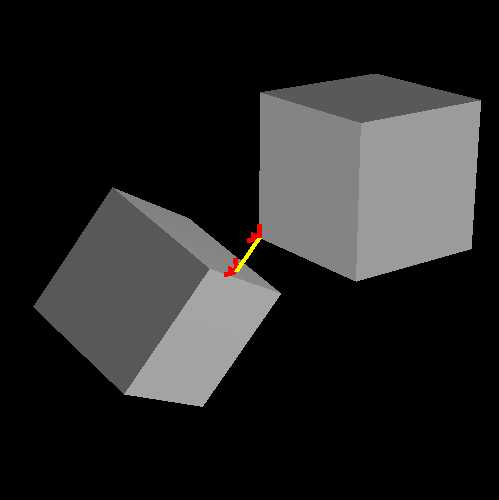
\includegraphics[width=0.50\columnwidth]{fig/collision.jpg}
    \caption{Collision detection}
  \end{center}
\end{figure}

\subsubsection{Robot Motion and Interference Calculation}
When performing a static simulation of the action of grabbing an object with the hand, it is possible to investigate the interference between the links of the hand (fingers) and the target object, and stop the action of grabbing the object when this occurs.

{\baselineskip=10pt
\begin{verbatim}
(load "irteus/demo/sample-arm-model.l")
(setq *sarm* (instance sarmclass :init))
(send *sarm* :reset-pose)
(setq a 42)
(send *sarm* :move-fingers a)
(setq *target* (make-cube 30 30 30))
(send *target* :translate #f(350 200 400))
(objects (list *sarm* *target*))

(send *sarm* :inverse-kinematics *target* :move-target (send *sarm* :end-coords) :debug-view t)
(while (> a 0)
  (if (collision-check-objects
       (list (send *sarm* :joint-fr :child-link)
             (send *sarm* :joint-fl :child-link))
       (list *target*))
      (return))
  (decf a 0.1)
  (send *irtviewer* :draw-objects)
  (send *sarm* :move-fingers a))
(send *sarm* :end-coords :assoc *target*)

(dotimes (i 100)
  (send *sarm* :joint0 :joint-angle 1 :relative t)
  (send *irtviewer* :draw-objects))
(send *sarm* :end-coords :dissoc *target*)
(dotimes (i 100)
  (send *sarm* :joint0 :joint-angle -1 :relative t)
  (send *irtviewer* :draw-objects))
\end{verbatim}
}

Similar functionality is provided by the methods :open-hand and :close-hand in the "irteus/demo/sample-arm-model.l" file.

\subsection{Interference Calculation by PQP}

PQP is an interference calculation library developed by Lin et al.'s group at the University of North Carolina. The usage of the PQP software package is described in irteus/PQP/README.txt, and can be understood by reading irteus/PQP/src/PQP.h.

The files for using PQP with irteus consist of CPQP.C, euspqp.c, and pqp.l.
To determine if two geometric models will collide,
{\baselineskip=10pt
\begin{verbatim}
(defun pqp-collision-check (model1 model2
				       &optional (flag PQP_FIRST_CONTACT) &key (fat 0) (fat2 nil))
  (let ((m1 (get model1 :pqpmodel))  (m2 (get model2 :pqpmodel))
        (r1 (send model1 :worldrot)) (t1 (send model1 :worldpos))
        (r2 (send model2 :worldrot)) (t2 (send model2 :worldpos)))
    (if (null fat2) (setq fat2 fat))
    (if (null m1) (setq m1 (send model1 :make-pqpmodel :fat fat)))
    (if (null m2) (setq m2 (send model2 :make-pqpmodel :fat fat2)))
    (pqpcollide r1 t1 m1 r2 t2 m2 flag)))
\end{verbatim}
}
should be called. 
r1,r1,r2,t1 are the translation vector and rotation matrix of each object, and (get model1 :pqpmodel) refers to the pointer to the PQP geometric model. This pointer is computed in the :make-pqpmodel method as follows.
{\baselineskip=10pt
\begin{verbatim}
(defmethod cascaded-coords
  (:make-pqpmodel
   (&key (fat 0))
   (let ((m (pqpmakemodel))
         vs v1 v2 v3 (id 0))
     (setf (get self :pqpmodel) m)
     (pqpbeginmodel m)
     (dolist (f (send self :faces))
       (dolist (poly (face-to-triangle-aux f))
         (setq vs (send poly :vertices)
               v1 (send self :inverse-transform-vector (first vs))
               v2 (send self :inverse-transform-vector (second vs))
               v3 (send self :inverse-transform-vector (third vs)))
         (when (not (= fat 0))
           (setq v1 (v+ v1 (scale fat (normalize-vector v1)))
                 v2 (v+ v2 (scale fat (normalize-vector v2)))
                 v3 (v+ v3 (scale fat (normalize-vector v3)))))
         (pqpaddtri m v1 v2 v3 id)
         (incf id)))
     (pqpendmodel m)
     m)))
\end{verbatim}
}
Here, (pqpmakemodel) is called first.
In pqpmakemodel, defined in euqpqp.c,

{\baselineskip=10pt
\begin{verbatim}
pointer PQPMAKEMODEL(register context *ctx, int n, register pointer *argv)
{
    int addr = PQP_MakeModel();
    return makeint(addr);
}
\end{verbatim}
}

is invoked, which is the same as in CPQP.C
{\baselineskip=10pt
\begin{verbatim}
PQP\_Model *PQP_MakeModel()
{
    return new PQP_Model();
}
\end{verbatim}
}
PQP\_Model() is defined in PQP.h. After the functions in euslisp are passed to the actual PQP library functions in this way, an instance of the PQP geometric model is created with (pqpbeginmodel m) and the surface information is registered as (pqpaddtri m v1 v2 v3 id) to register the surface information.

\input{pqp-func}

\subsection{Interference Calculation with Bullet}

Bullet is a physics engine, and as part of it, an interference calculation function is provided.
The files for using Bullet with irteus consist of CBULLET.cpp, eusbullet.c, and bullet.l.
The calling order inside the function is the same as PQP.

The differences between PQP and Bullet are as follows.
\begin{itemize}
  \item If you call collision-distance when there is interference, PQP will return 0 as the distance and a meaningless point as the closest point. Bullet, on the other hand, returns the shortest distance (called penetration depth) that should be moved to eliminate interference as the distance. Also, as the closest point, the points at both ends of the shortest distance to eliminate interference are returned.
  \item PQP can handle non-convex mesh models as is, but Bullet internally computes and handles the convex hull of non-convex models.
\end{itemize}

\input{bullet-func}

%% irtcollision.l
%% pqp.l
%% bullet.l

\section{BVH Data}
 \input{irtbvh-func}

\section{Collada Data}
 \input{irtcollada-func}

\section{Point Cloud Data}
 \input{irtpointcloud-func}

\section{Graph Representation}
 \input{irtgraph-func}


%% irtbvh.l
%% irtcollada.l
%% irtgraph.l
%% irtimage.l
%% irtpointcloud.l
%% png.l

\section{irteus Extension}
 \subsection{GL/X Display}
  \input{irtgl-func}
  \input{irtx-func}
 \subsection{Utility Function}
 \input{irtutil-func}
 \input{gnuplotlib-func}
 \subsection{Math Function}
 \input{irtmath-func}
 \subsection{Image Function}
 \input{irtimage-func}
 \input{png-func}

%% irtgl.l
%% irtutil.l
%% irtviewer.l
%% irtx.l
%% irtmath.l


\cleardoublepage
\markboth{Euslisp version \eusversion Reference Manual}{Index}
\footnotesize
\printindex
\end{document}

